
In order to verify the feasibility of the proposed load balancer architecture, the author evaluated the performance levels of the load balancer with the following criteria;
(1) Performance analysis:
The author evaluated the basic characteristics of the load balancer using physical servers in the on-premise data center, and compared performance levels with those of iptables DNAT and nginx as a load balancer.
(2) Portability:
The author also carried out the same performance measurement in GCP and AWS to show the containerized ipvs load balancer is runnable in the cloud environment.
(3) Redundancy and Scalability:
The author evaluated ECMP functionality by monitoring routing table updates on the router when the new load balancer is added or removed.
The author also evaluated the aggregated performance level of the ECMP redundant load balancer.

\section{Performance analysis of proposed load balancer}

\subsubsection{Experimental conditions}

Throughput measurements were carried out in order to examine the basic characteristics of the containerized ipvs load balancer in an on-premise data center.
Figure~\ref{fig:benchmark-schem} shows the schematic diagram of the experimental setup for the measurement.
A benchmark program called wrk\cite{Glozer2016} were used.
Multiple nginx {\em pods} are deployed on multiple nodes as web servers in the Kubernetes cluster.
In each nginx {\em pod}, single nginx web server program that returns the IP address of the {\em pod} itself is running.
The author then launched ipvs pod and nginx pod as load balancers on one of the nodes, after that, performed the throughput measurement changing the number of the nginx web server pods.
On every Kubernetes node, there are iptables DNAT rules that function as an internal load balancer.
The author also measured throughput for the iptables DNAT as a load balancer.
The throughput is measured by sending out HTTP requests from the wrk towards a load balancer and by counting the number of responses the benchmark client received.

\begin{figure}[h]
  \centering
  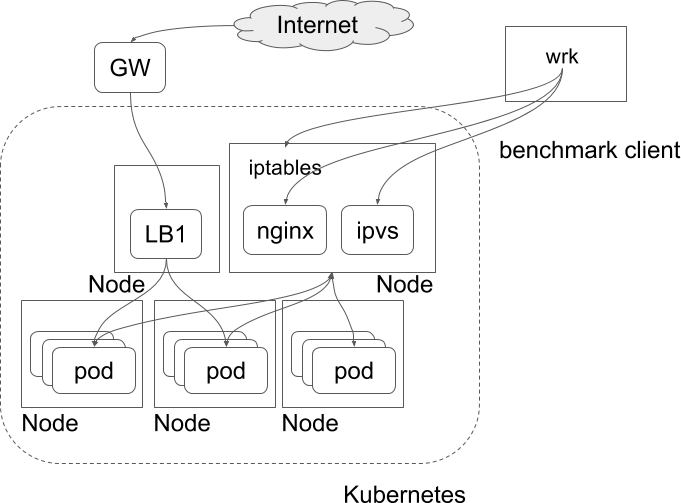
\includegraphics[width=0.8\columnwidth]{Figs/benchmark-schem}
  \par\bigskip
  \centering
  \begin{minipage}{0.9\columnwidth}
    \caption[Benchmark setup]{
      Benchmark setup.
      There are nodes on which nginx pods are deployed as web servers.
      There is another node where ipvs pod and nginx pod are deployed.
      Iptables DNAT rules exist on every Kubernetes node as an internal load balancer.
      Throughput measurements are performed against ipvs pod, nginx pod, and iptables DNAT rules.
      Each of the load balancers distributes the packets from the wrk to the nginx web servers.
      The response packets from the nginx web servers follow the same route as the request packets.  
    }
    \label{fig:benchmark-schem}
  \end{minipage}
\end{figure}

Table~\ref{fig:benchmark-schem} shows an example of the command-line for the benchmark program, wrk, and the corresponding output.
The command-line in Table~\ref{tab:bench_example} will generate 40 wrk program threads
and allow those threads to send out a total of 800 concurrent HTTP requests over the period of 30 seconds.
The output example shows information including per-thread statistics, error counts, throughput in [Request/sec] and data rate in [Transfer/sec].


{
%\setlength{\tabcolsep}{3em}
\renewcommand{\arraystretch}{1.1}

\begin{table}[h]

  \begin{subtable}{1\textwidth}
    \centering
    \begin{tabular}{lll}
      \hline
      &\verb|  wrk -c800 -t40 -d30s http://172.16.72.2:8888/       |& \\
      &\verb|      -c: concurrency, -t: # of thread, -d: duration  |& \\
      \hline
    \end{tabular}
    \centering\caption{Command line}
  \end{subtable}
 
\par\bigskip
 
  \begin{subtable}{1\textwidth}
    \centering
    \begin{tabular}{lll}
      \hline
      &\verb| Running 30s test @ http://10.254.0.10:81/            |& \\ 
      &\verb|  40 threads and 800 connections                      |& \\
      &\verb|  Thread Stats   Avg      Stdev     Max   +/- Stdev   |& \\
      &\verb|    Latency    15.82ms   41.45ms   1.90s    91.90\%   |& \\
      &\verb|    Req/Sec     4.14k   342.26     6.45k    69.24\%   |& \\
      &\verb|  4958000 requests in 30.10s, 1.14GB read             |& \\
      &\verb|  Socket errors: connect 0, read 0, write 0, timeout 1|& \\
      &\verb|Requests/sec: 164717.63                               |& \\
      &\verb|Transfer/sec:     38.86MB                             |& \\
      \hline
    \end{tabular}
    \centering\caption{Output example}
  \end{subtable}

  \centering
  \begin{minipage}{0.9\columnwidth}
    \caption[Benchmark command line and output example]{
      Benchmark command line and output example.
      (a) This command line will generate 40 wrk program threads and allow those threads to send out a total of 800 concurrent HTTP requests over the period of 30 seconds.
      (b) The output example shows information including per-thread statistics, error counts, throughput in [Request/sec] and data rate in [Transfer/sec].
      The throughput is 164717.63 [Request/sec] in this example.
    }
    \label{tab:bench_example}
  \end{minipage}
\end{table}
}

{
\setlength{\tabcolsep}{2em}
\renewcommand{\arraystretch}{1.1}

\begin{table}[h]
  \centering
  \begin{tabular}{ll}
    \hline 
    \multicolumn{2}{l}{[Hardware Specification]}   \\
    & CPU: Xeon E5-2450 2.10GHz (with 8 core, Hyper Threading) \\
    & Memory: 32GB \\
    & NIC: Broadcom BCM5720 with 4 rx-queues, 1 Gbps \\
    & (Node x 6, Load Balacner x 1, Client x 1) \\
%    \hline 
    & \\
%    \hline 
    \multicolumn{2}{l}{[Node Software]}  \\
    & OS: Debian 8.7, linux-3.16.0-4-amd64 \\
    & Kubernetes v1.10.6 \\
    & flannel v0.7.0 \\
    & etcd version: 3.0.15 \\
%    \hline 
    & \\
%    \hline 
    \multicolumn{2}{l}{[Container Software]}   \\
    & Keepalived: v1.3.2 (12/03,2016) \\
    & nginx : 1.11.1(load balancer), 1.13.0(web server) \\
    \hline
  \end{tabular}

  \centering
  \begin{minipage}{0.9\columnwidth}
    \caption[Hardware and software specifications]{
      Hardware and software specifications.
      The hardware had eight physical CPU cores and a network interface card (NIC) with four rx-queues.
    }
    \label{tab:hw_machine_spec}
  \end{minipage}
\end{table}
}

Table~\ref{tab:hw_machine_spec} shows hardware and software configuration used in the experiment.
The author used a total of eight servers; six servers for Nodes, one for the load balancer and one for the benchmark client, with all having the same hardware specifications.
The hardware had eight physical CPU cores and a network interface card (NIC) with four rx-queues.
The author configured nginx HTTP server to return a small HTTP content, the IP address of the {\em pod}, to make a relatively severe condition for load balancers. 
The size of the character string making up an IP address is limited to 15 bytes.

The author also investigated the performance level, varying two types of network conditions:
The first condition is the setting for multicore packet processing.
It is known that distributing handling of interrupts from the NIC and the subsequent IP protocol processing, among multiple cores impact the network performance.
To derive the best performance from load balancers, the author investigated how this setting would affect their performance levels.
The second condition is an overlay network setting\cite{Sill2016,Marmol2015}.
The overlay network is often used to build the Kubernetes cluster and therefore used in the experiment.
Flannel\cite{CoreOSFlannel} is one of the popular overlay network technologies. 
The author compared the performance levels of three backends settings\cite{CoreOSFlannelBackend} of flannel, i.e., operating modes, to find the best setting.

\FloatBarrier

\subsubsection{Effect of multicore proccessing}

Figure~\ref{fig:ipvs_mcore_proccessing} shows the result of the throughput measurement for the ipvs load balancer with different multicore processing settings.
Since hardware used in the experiment has a NIC with four rx-queues, and a CPU with eight cores,
the setting \enquote{(RSS, RPS) = (on, off)} uses 4 cores and \enquote{(RSS, RPS) = (off, on)} uses 8 cores for packet processing.
For the setting \enquote{(RSS, RPS) = (off, off)}, only one core is used for the packet processing.

There is a general trend in the throughput result, where the throughput linearly increases as the number of nginx {\em pod}s increases and then it eventually saturates.
For example, if we look at the red line in the Figure~\ref{fig:ipvs_mcore_proccessing}, the throughput increases almost linearly with the increasing number of the nginx pods(web servers) from 1 to around 14, and then saturated.
The increase indicates that the load balancer functions properly, as the load balancer increased throughput by distributing HTTP requests to multiple of the web servers.
%
The saturated throughput indicates the maximum performance level of the load balancer, which could be determined either by network bandwidth between the benchmark client machine and the load balancer node, or CPU performance levels of these machines.
%
The maximum performance levels are dependent on the number of cores used for packet processing.
Throughput is highest for the setting with eight cores (rps is on), followed by four cores (rss is on), then single core (none).
This indicates that the more cores are used, the better the throughput is.

Figure~\ref{fig:iptables_mcore_proccessing} shows the result of the throughput measurement for iptables DNAT as a load balancer, with different multicore processing settings.
As is the case for the ipvs result, there is a general trend where the throughput increases as the number of nginx {\em pod}s increases and then it eventually saturates.
Also, throughput is highest for the setting with eight cores (rps is on), followed by four cores (rss is on), then single core (none).
%
The saturated performance levels of iptables DNAT and ipvs are the same for the condition with eight cores (rss is on). 
The saturated performance levels of iptables DNAT are higher than those of ipvs, for the conditions with four cores (rss is on) and single core (none).

\begin{figure}[h]
  \centering
  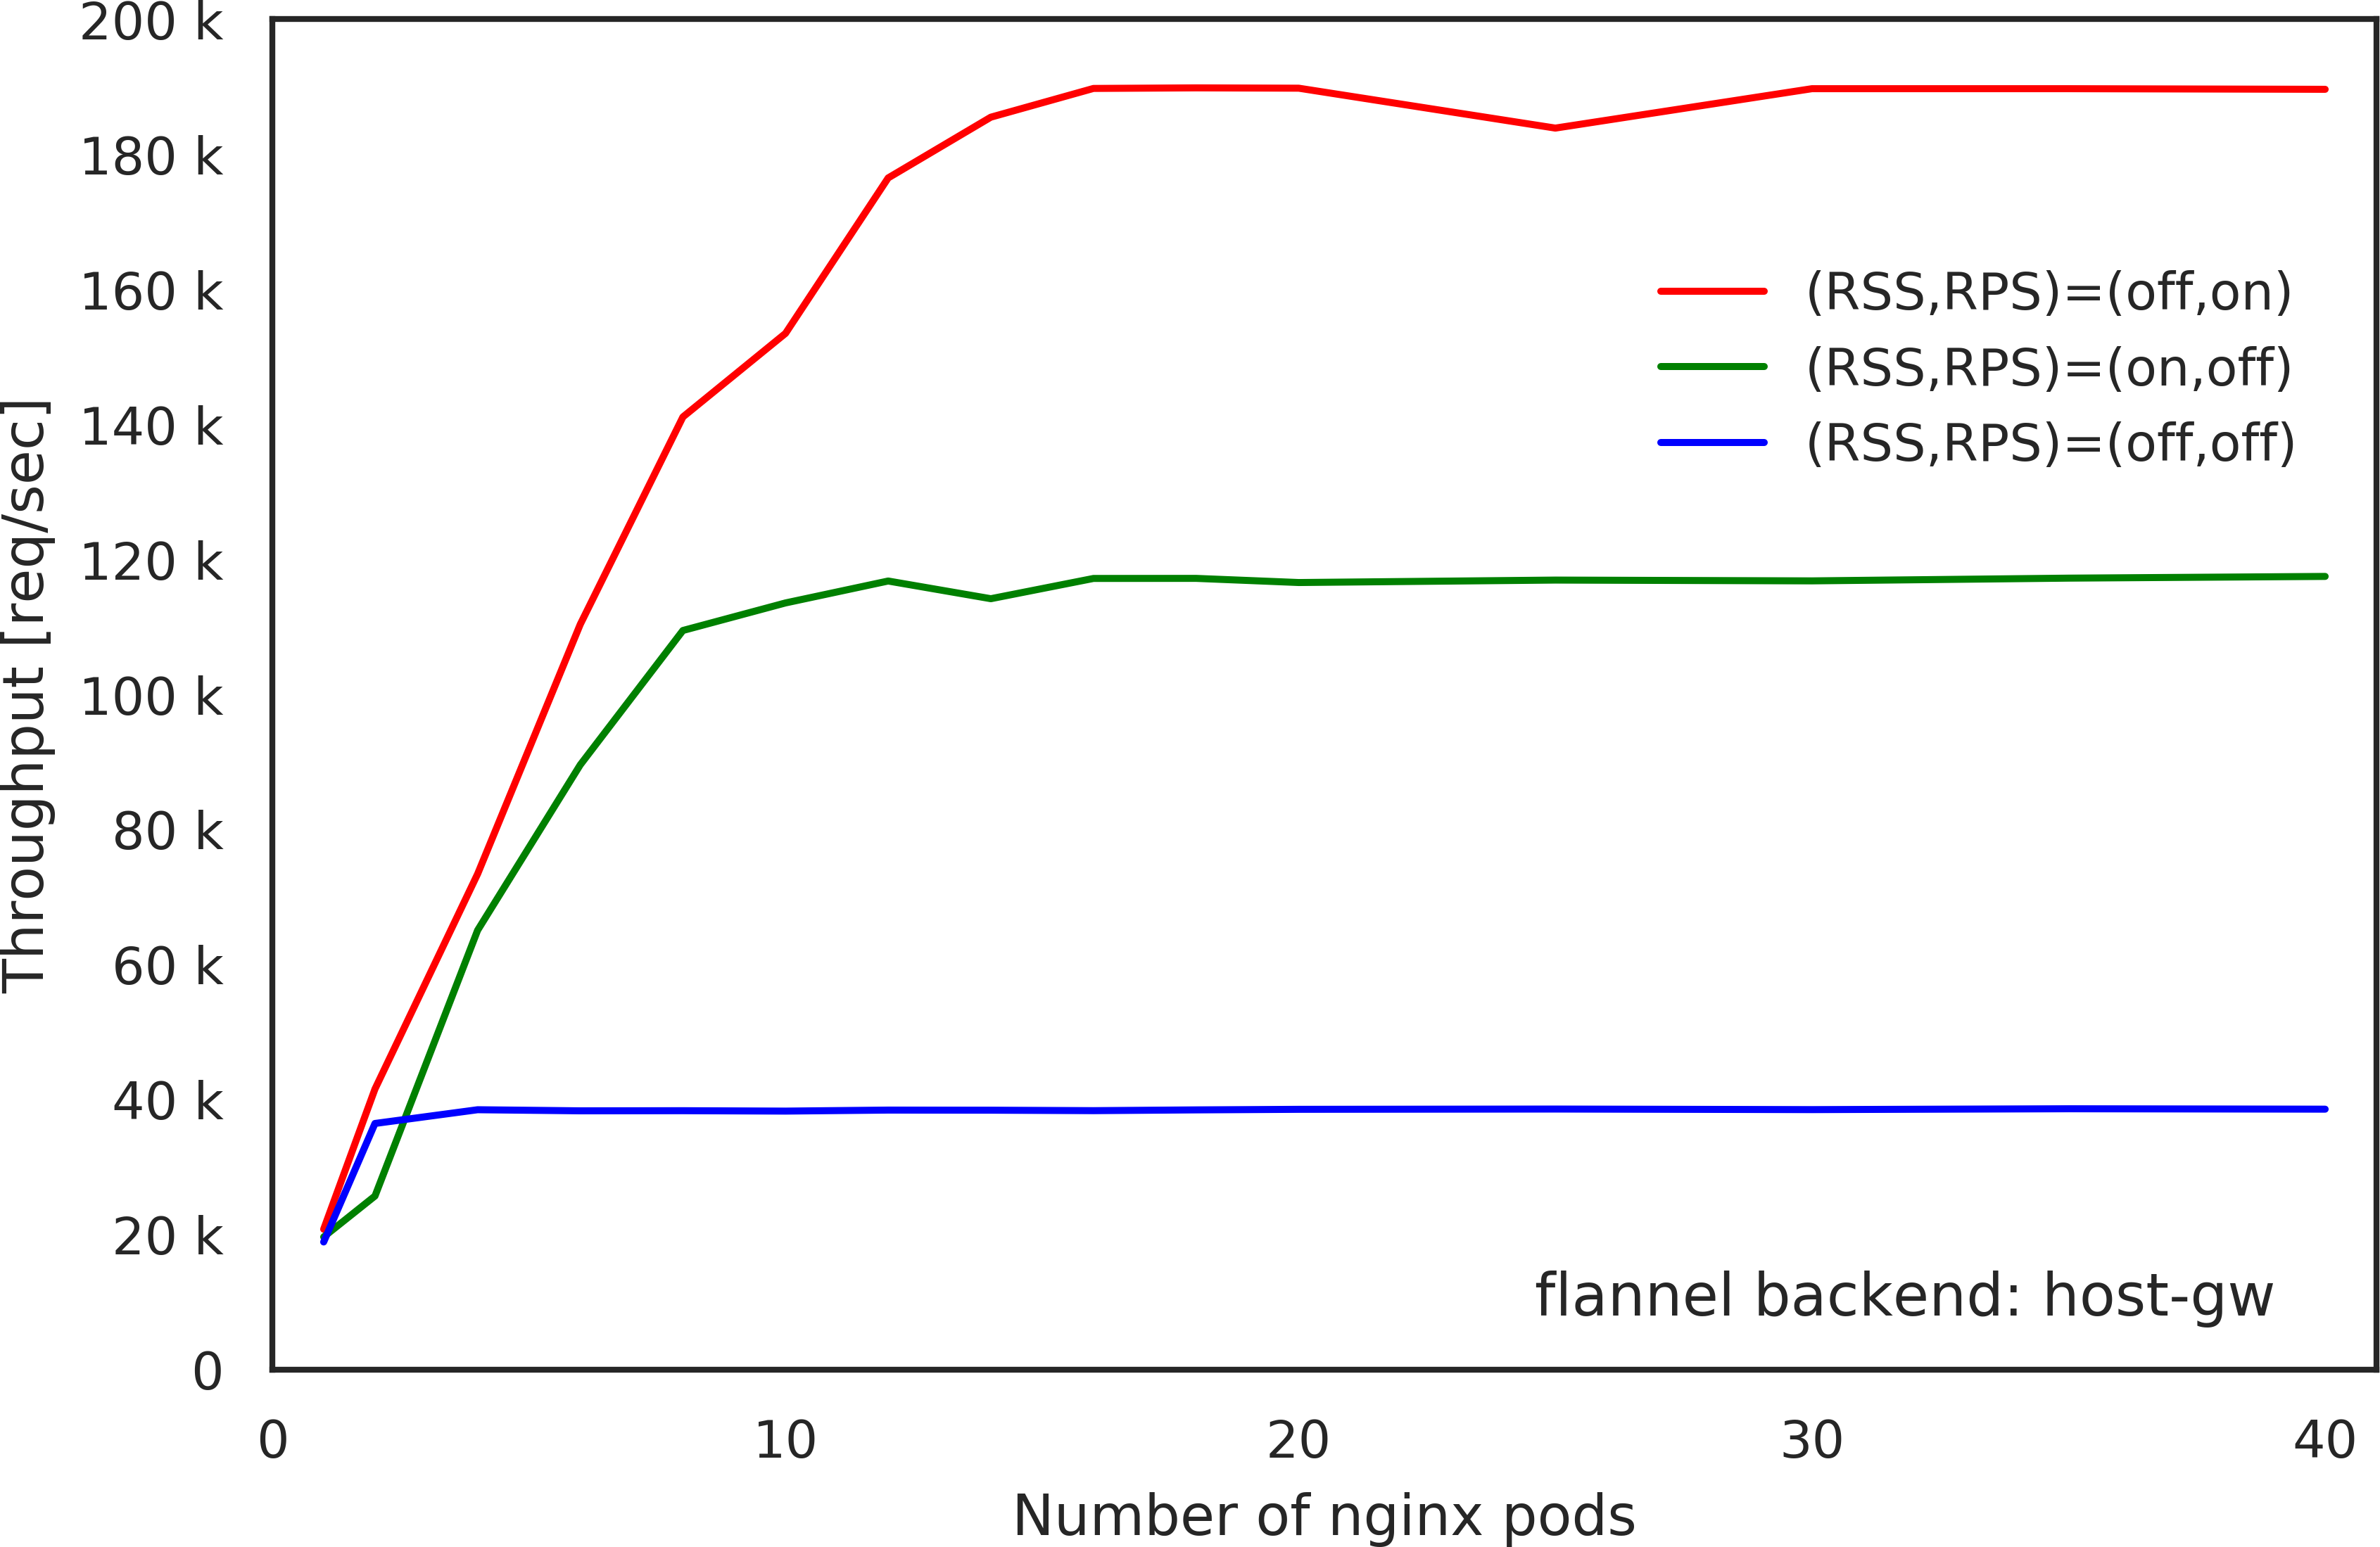
\includegraphics[width=0.75\columnwidth]{Figs/ipvs_mcore_proccessing}
  \par\bigskip
  \centering
  \begin{minipage}{0.9\columnwidth}
    \caption[Effect of multicore packet processing on ipvs throughput]{
Effect of multicore packet processing on ipvs throughput.
Throughput linearly increases as the number of nginx {\em pod}s increases and then it eventually saturates.
The throughput is highest for the setting with eight cores (rps is on), followed by four cores (rss is on), then single core (none).
    }
    \label{fig:ipvs_mcore_proccessing}
  \end{minipage}
\end{figure}


\begin{figure}[h]
  \centering
  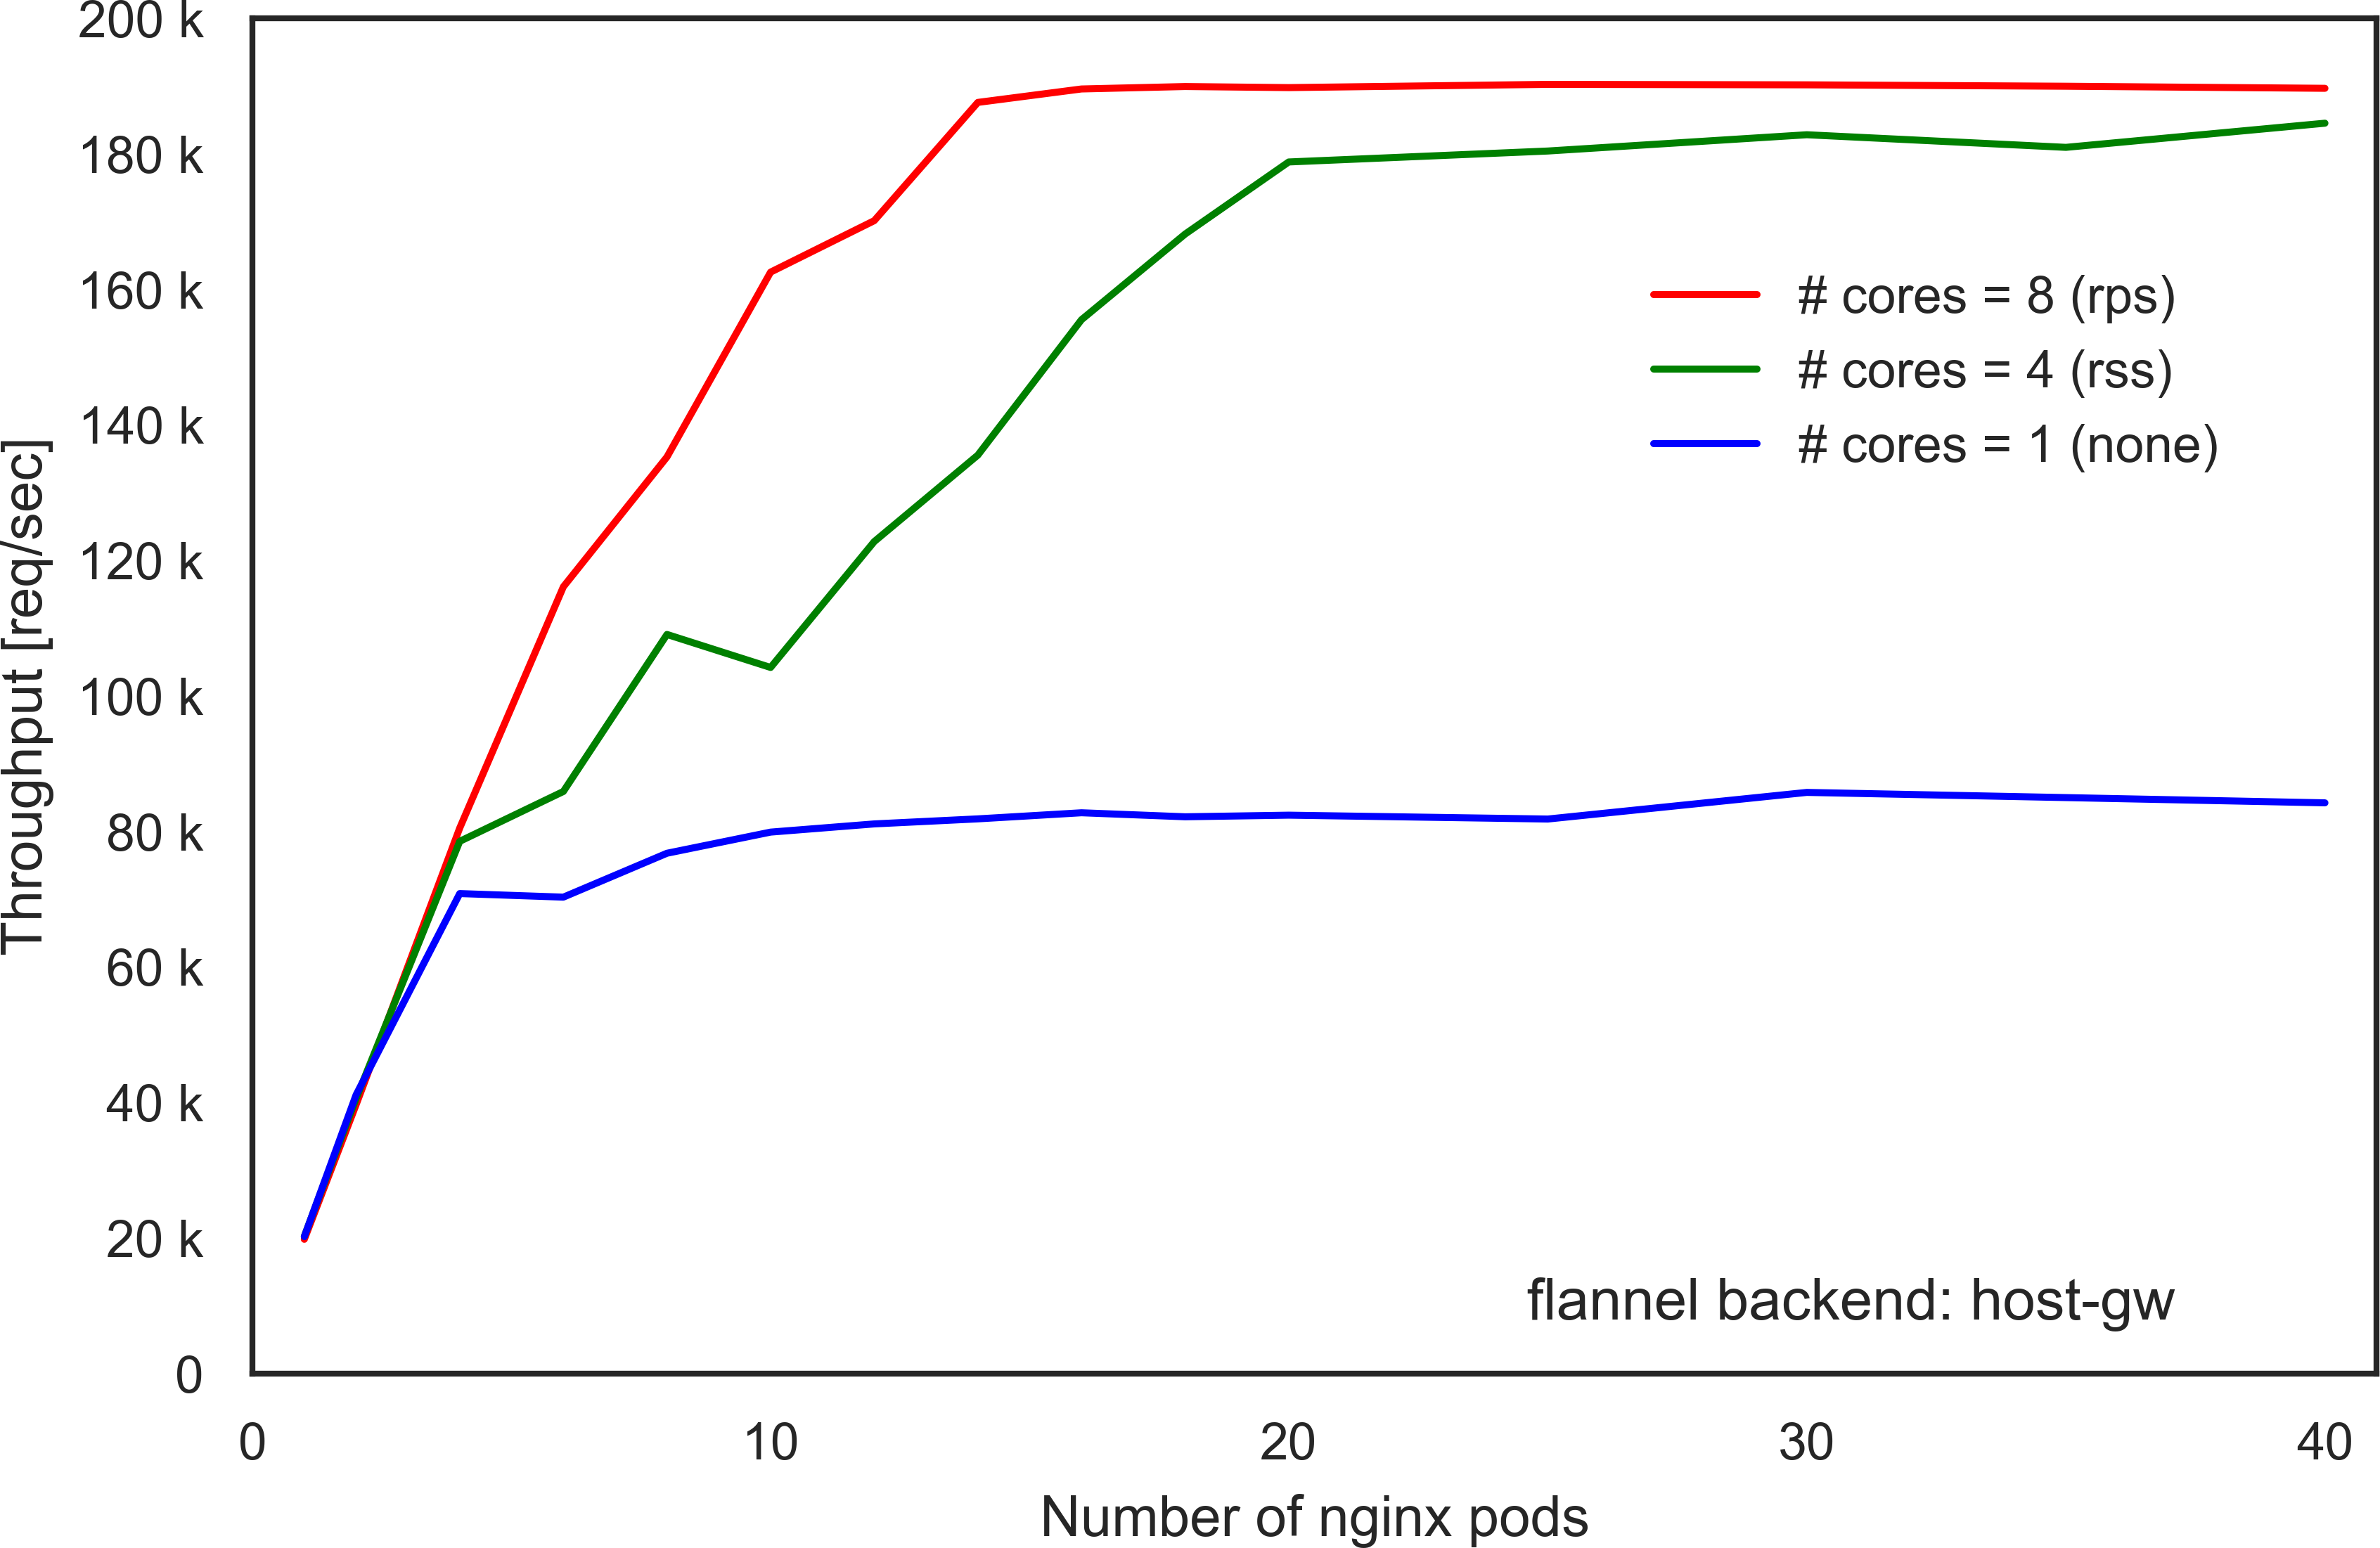
\includegraphics[width=0.75\columnwidth]{Figs/iptables_mcore_proccessing}
  \par\bigskip
  \centering
  \begin{minipage}{0.9\columnwidth}
    \caption[Effect of multicore packet processing on iptables DNAT throughput]{
Effect of multicore packet processing iptables DNAT throughput.
Throughput linearly increases as the number of nginx {\em pod}s increases and then it eventually saturates.
The throughput is highest for the setting with eight cores (rps is on), followed by four cores (rss is on), then single core (none).
    }
    \label{fig:iptables_mcore_proccessing}
  \end{minipage}
\end{figure}


\FloatBarrier

\subsubsection{Effect of overlay network}

Figure~\ref{fig:ipvs_flannel_mode} shows the ipvs throughput results for different overlay network settings.
The author used the flannel for the overlay network.
Flannel has three backend modes, host-gw, vxlan and udp, and the throughput for each setting are compared.

Except for the udp backend mode case, a general trend can be clearly seen, i.e., the throughput linearly increases as the number of nginx {\em pod} increases, and then it eventually saturates.
Among the flannel backend mode types, the host-gw mode where no encapsulation is conducted shows the highest performance level,
followed by the vxlan mode where the Linux kernel encapsulates the Ethernet frame.
The udp mode where flanneld itself encapsulates the IP packet shows significantly lower performances levels.

Figure~\ref{fig:iptables_flannel_mode} shows throughput results of the iptables DNAT as a load balancer for different overlay network settings.
The same characteristics can be seen for the iptables DNAT, although the performance level of the iptables DNAT for udp mode is slightly better than that of ipvs.

As is shown here, overlay network settings greatly affect the performance level.
The author considers the host-gw mode is the best, the vxlan tunnel the second best and the udp tunnel mode unusable.
In environments where containers need to communicate with each other via a gateway that has no knowledge of overlay network, the host-gw mode cannot be used, which is often the case in cloud environments. 
The author used host-gw mode for the rest of the experiments conducted in on-premise data centers and vxlan mode for the experiments conducted in cloud environments.

\begin{figure}[h]
  \centering
  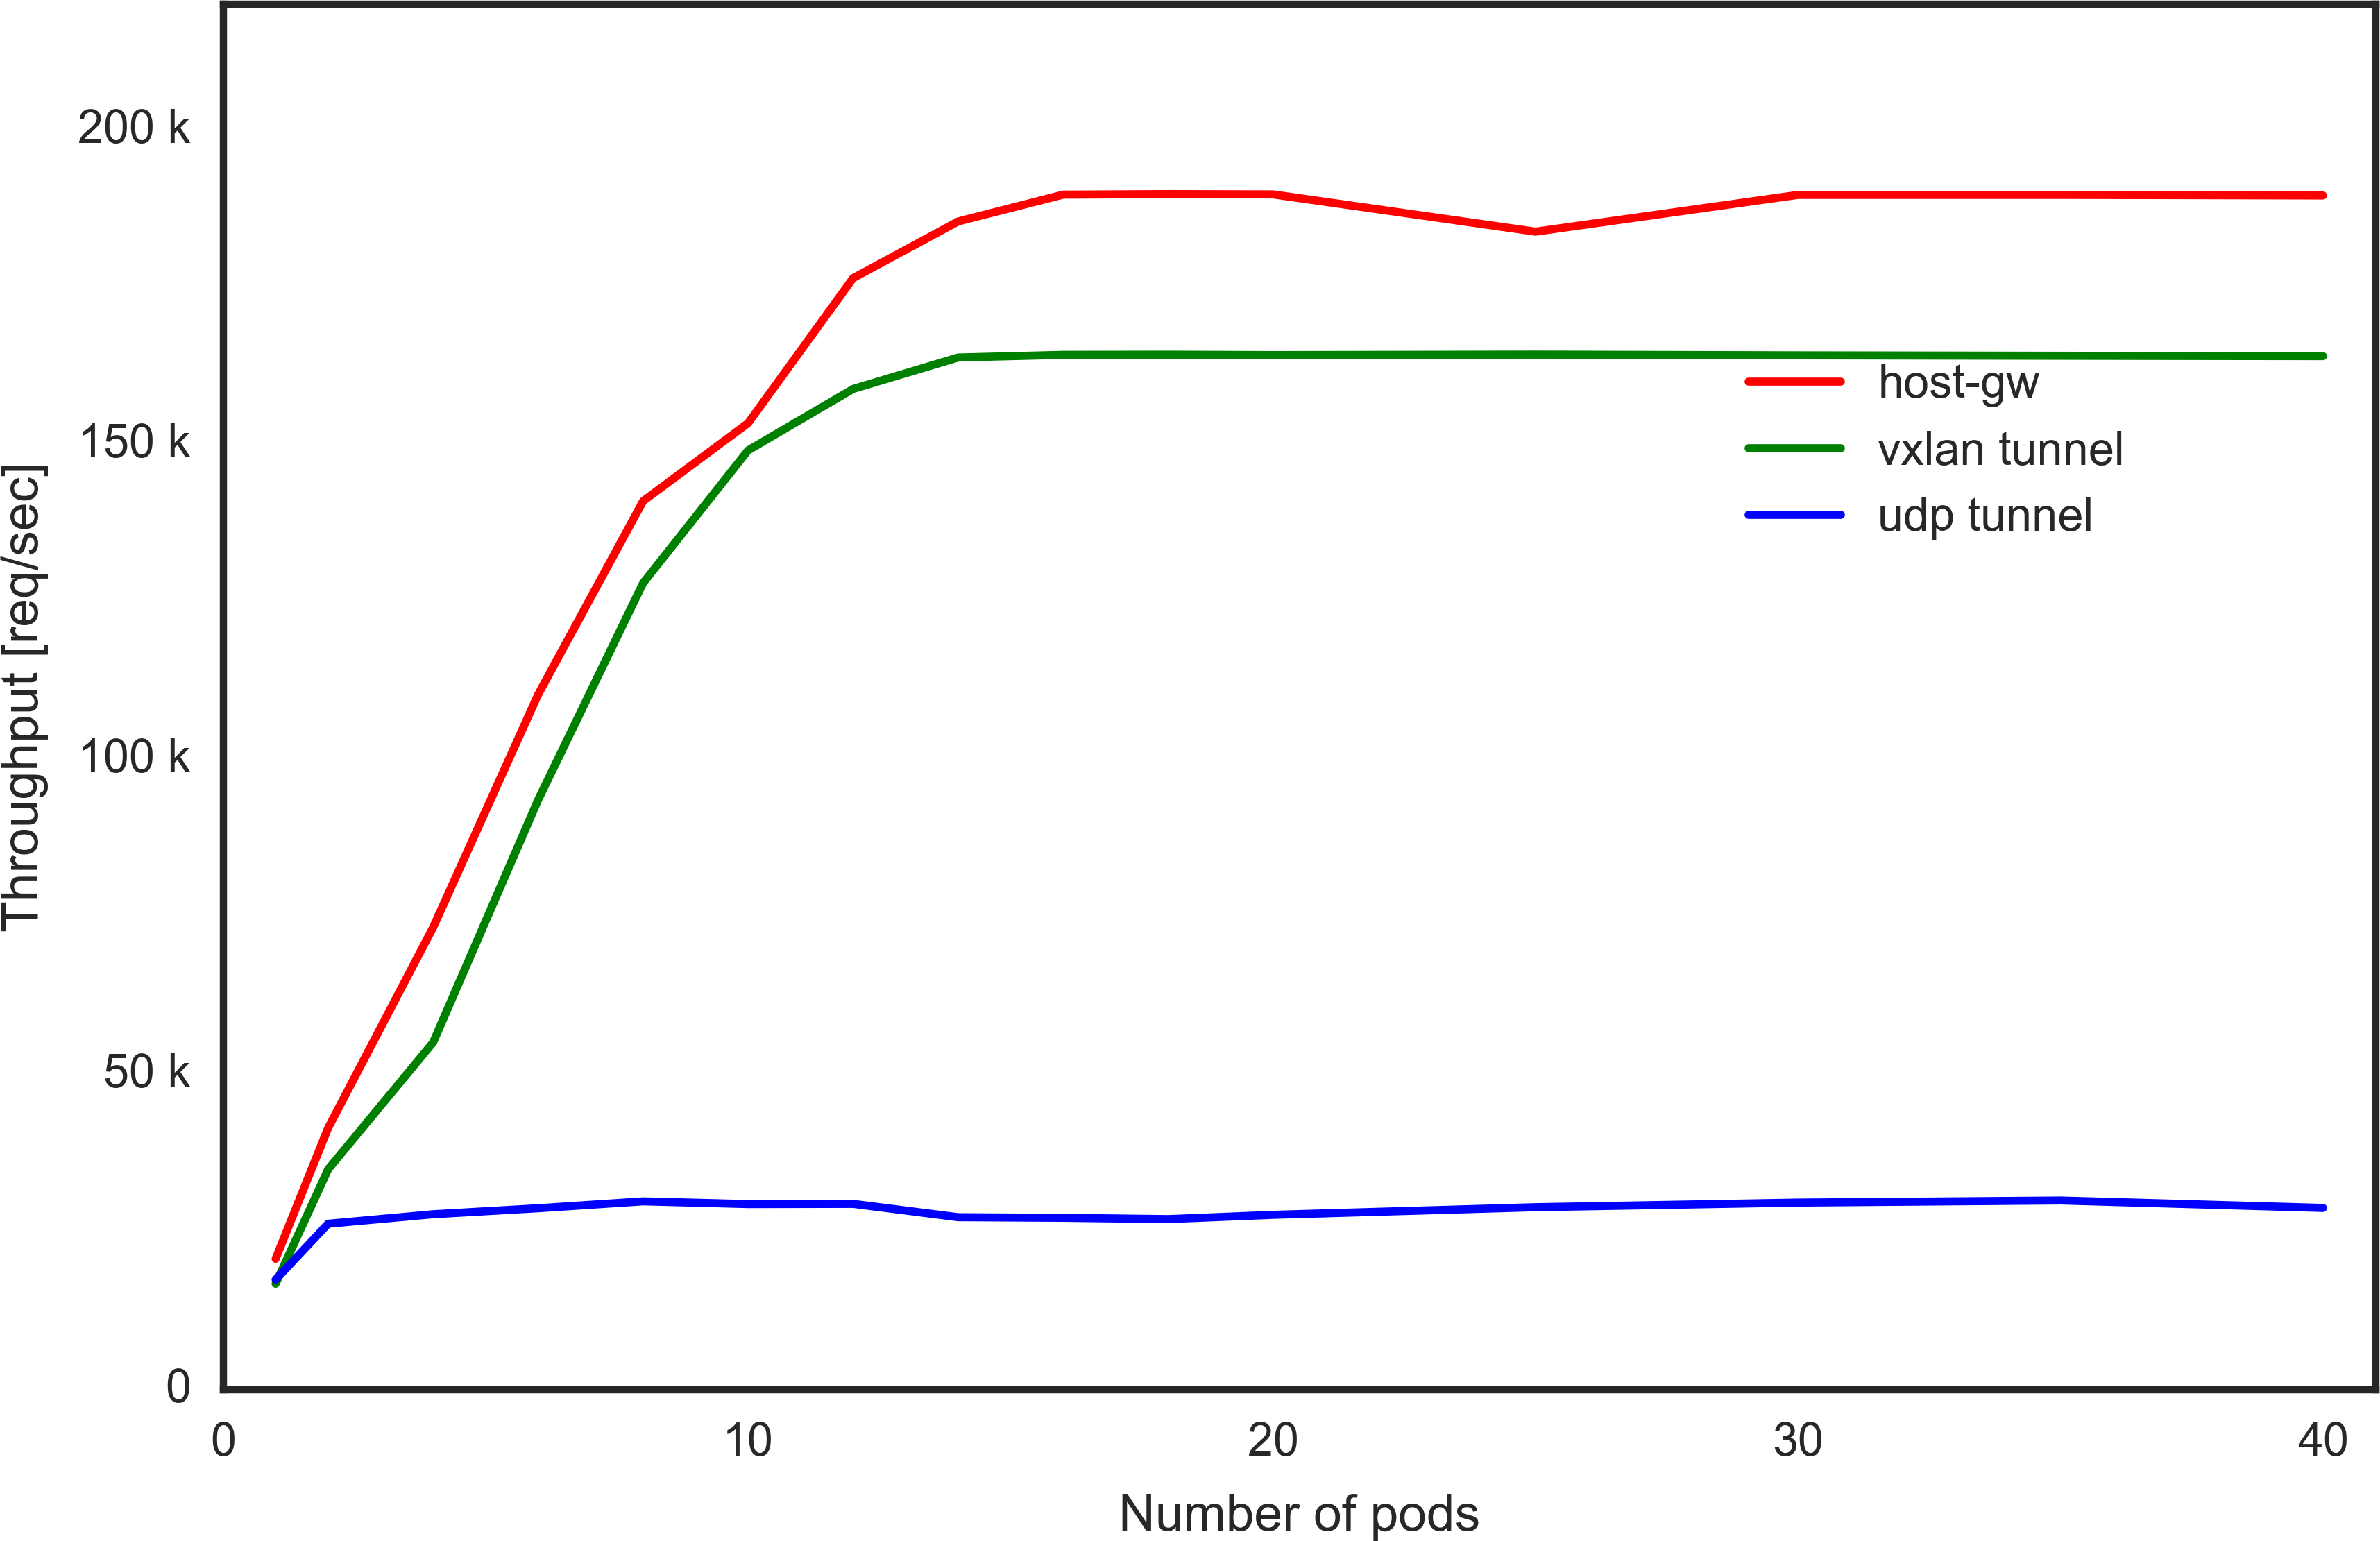
\includegraphics[width=0.75\columnwidth]{Figs/ipvs_flannel_mode}

  \par\bigskip
  \centering
  \begin{minipage}{0.9\columnwidth}
    \caption[Effect of flannel backend modes on ipvs throughput]{
      Effect of flannel backend modes on ipvs throughput.
      The host-gw mode shows the highest performance level, followed by the vxlan mode.
      The udp mode shows significantly lower performances levels.
    }
    \label{fig:ipvs_flannel_mode}
  \end{minipage}
\end{figure}

\begin{figure}[h]
    \centering
    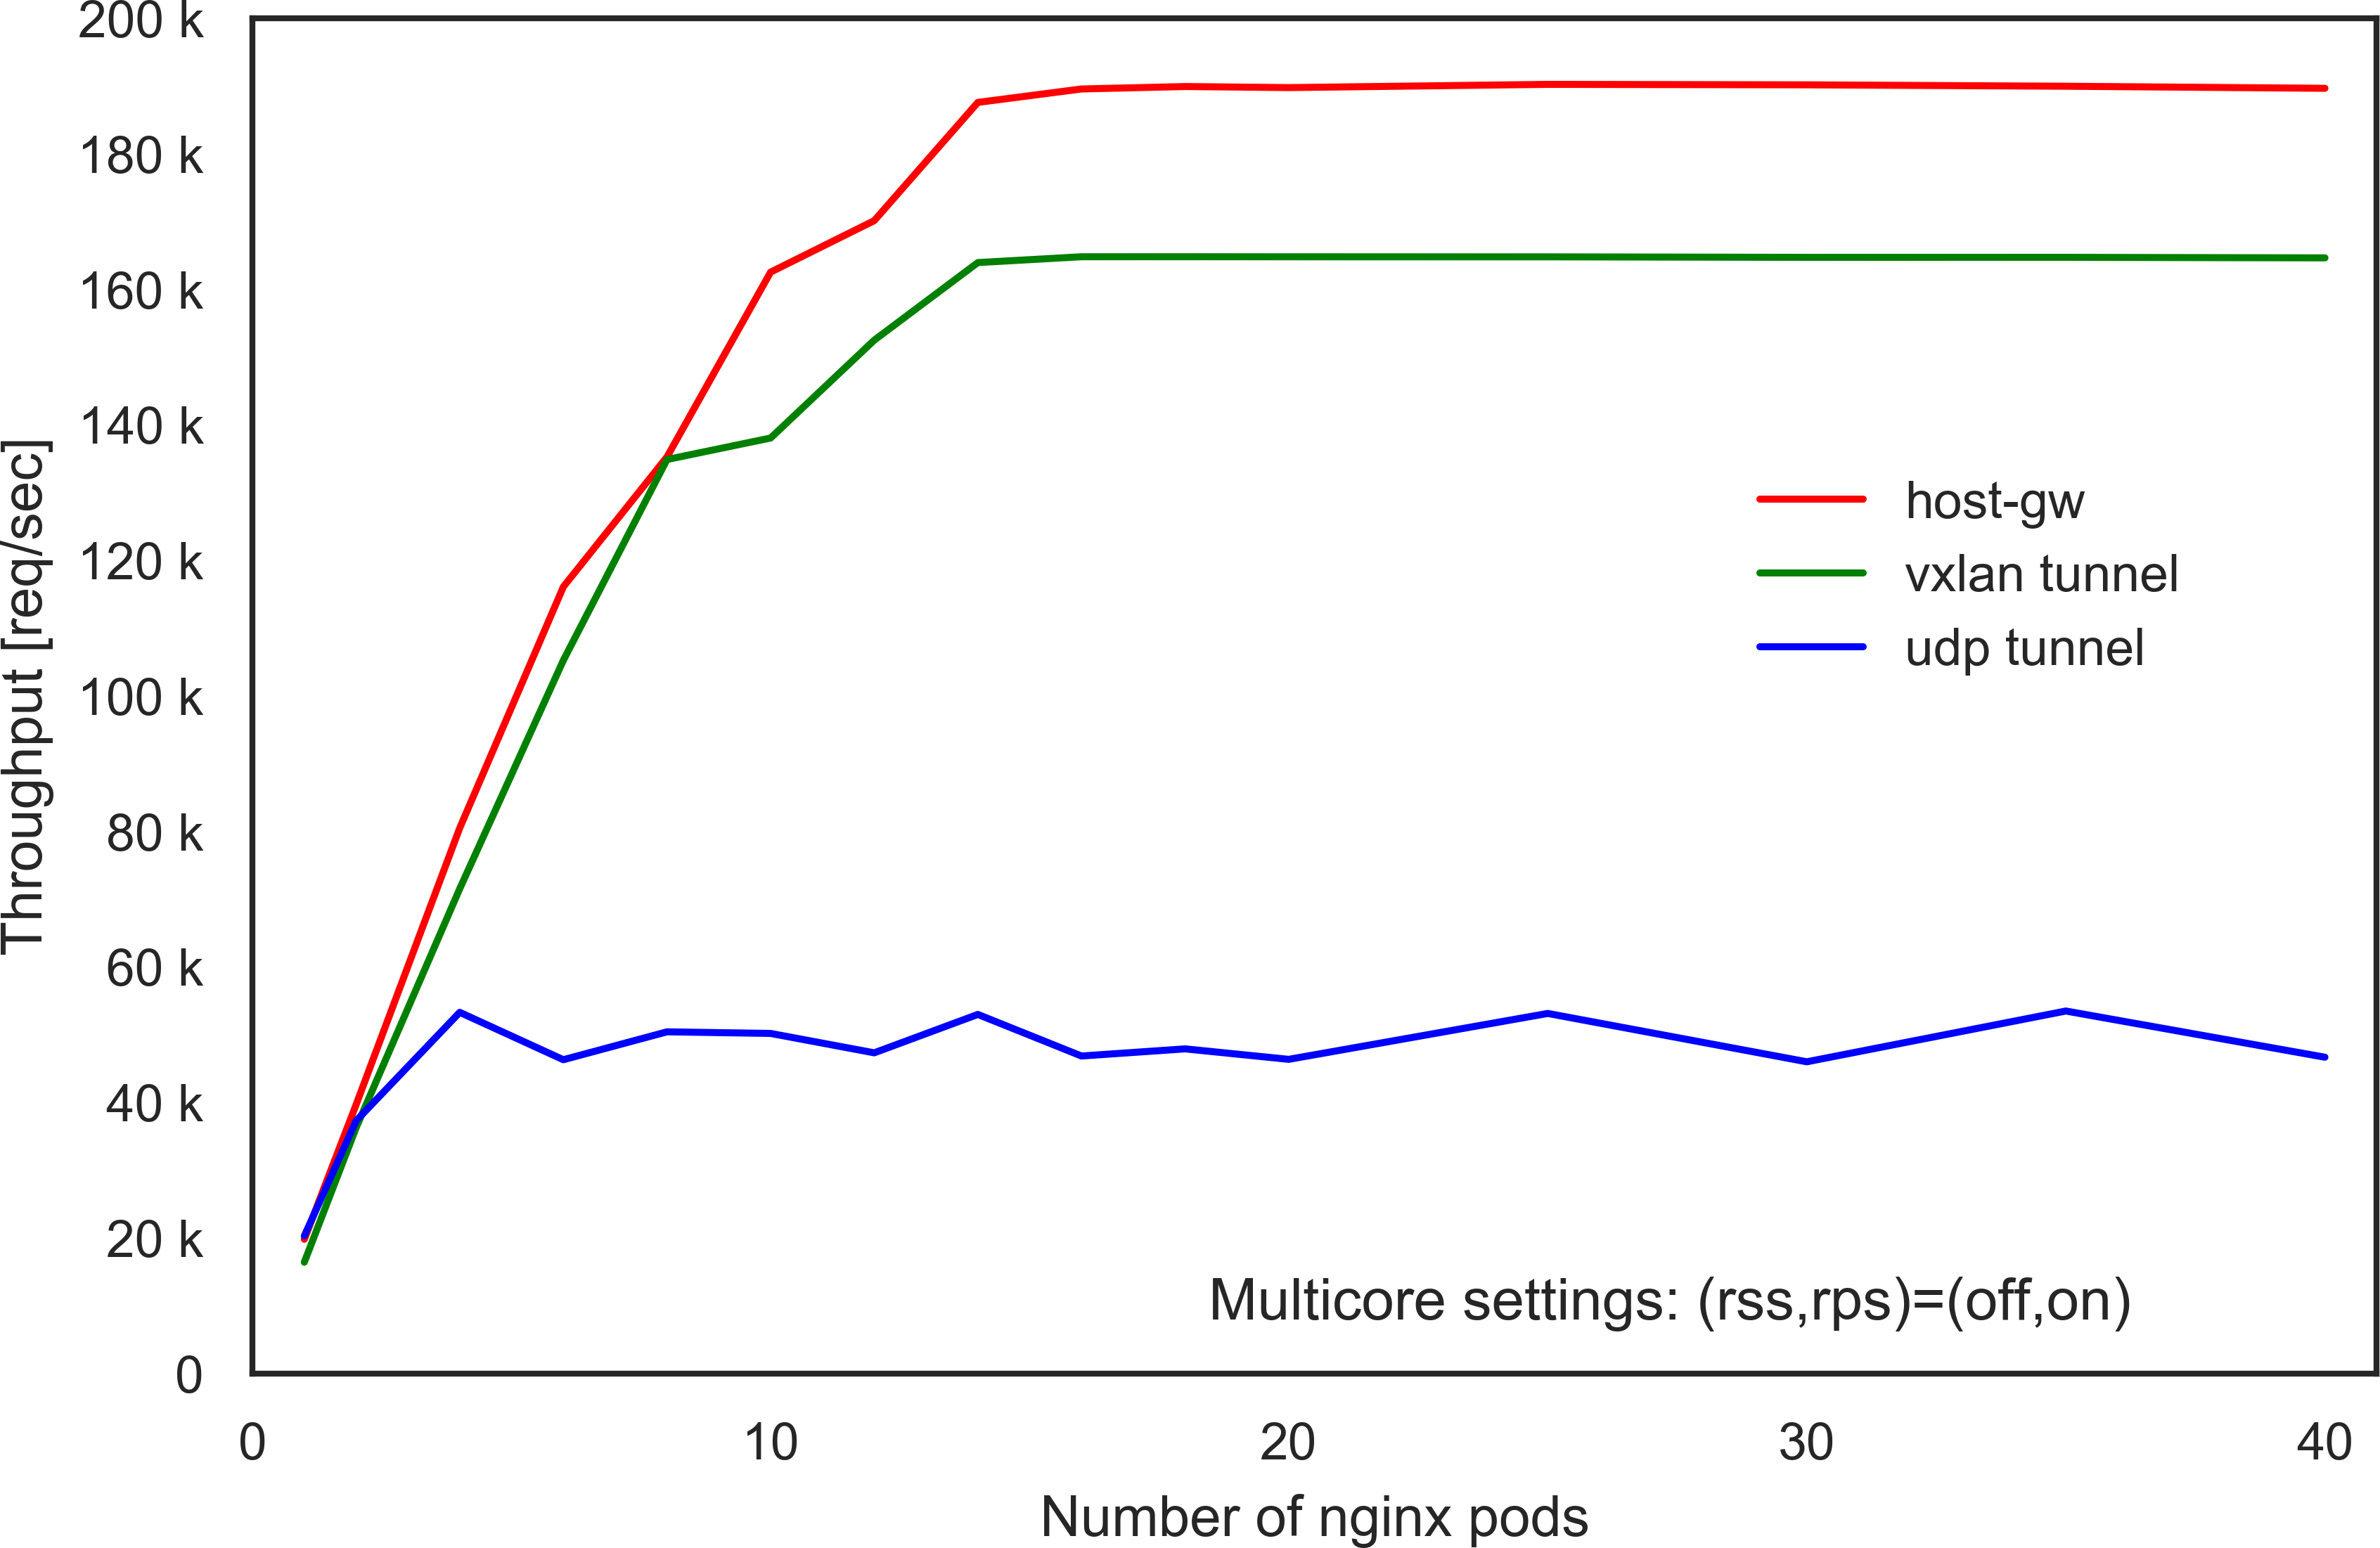
\includegraphics[width=0.75\columnwidth]{Figs/iptables_flannel_mode}

  \par\bigskip
  \centering
  \begin{minipage}{0.9\columnwidth}
    \caption[Effect of flannel backend modes on iptables DNAT throughput]{
      Effect of flannel backend modes on iptables DNAT throughput.
      the host-gw mode shows the highest performance level, followed by the vxlan mode.
      The udp mode shows significantly lower performances levels.
    }
    \label{fig:iptables_flannel_mode}
  \end{minipage}
\end{figure}

\FloatBarrier

\subsubsection{Comparison of different load balancer}

\begin{figure}[h]
  \centering
  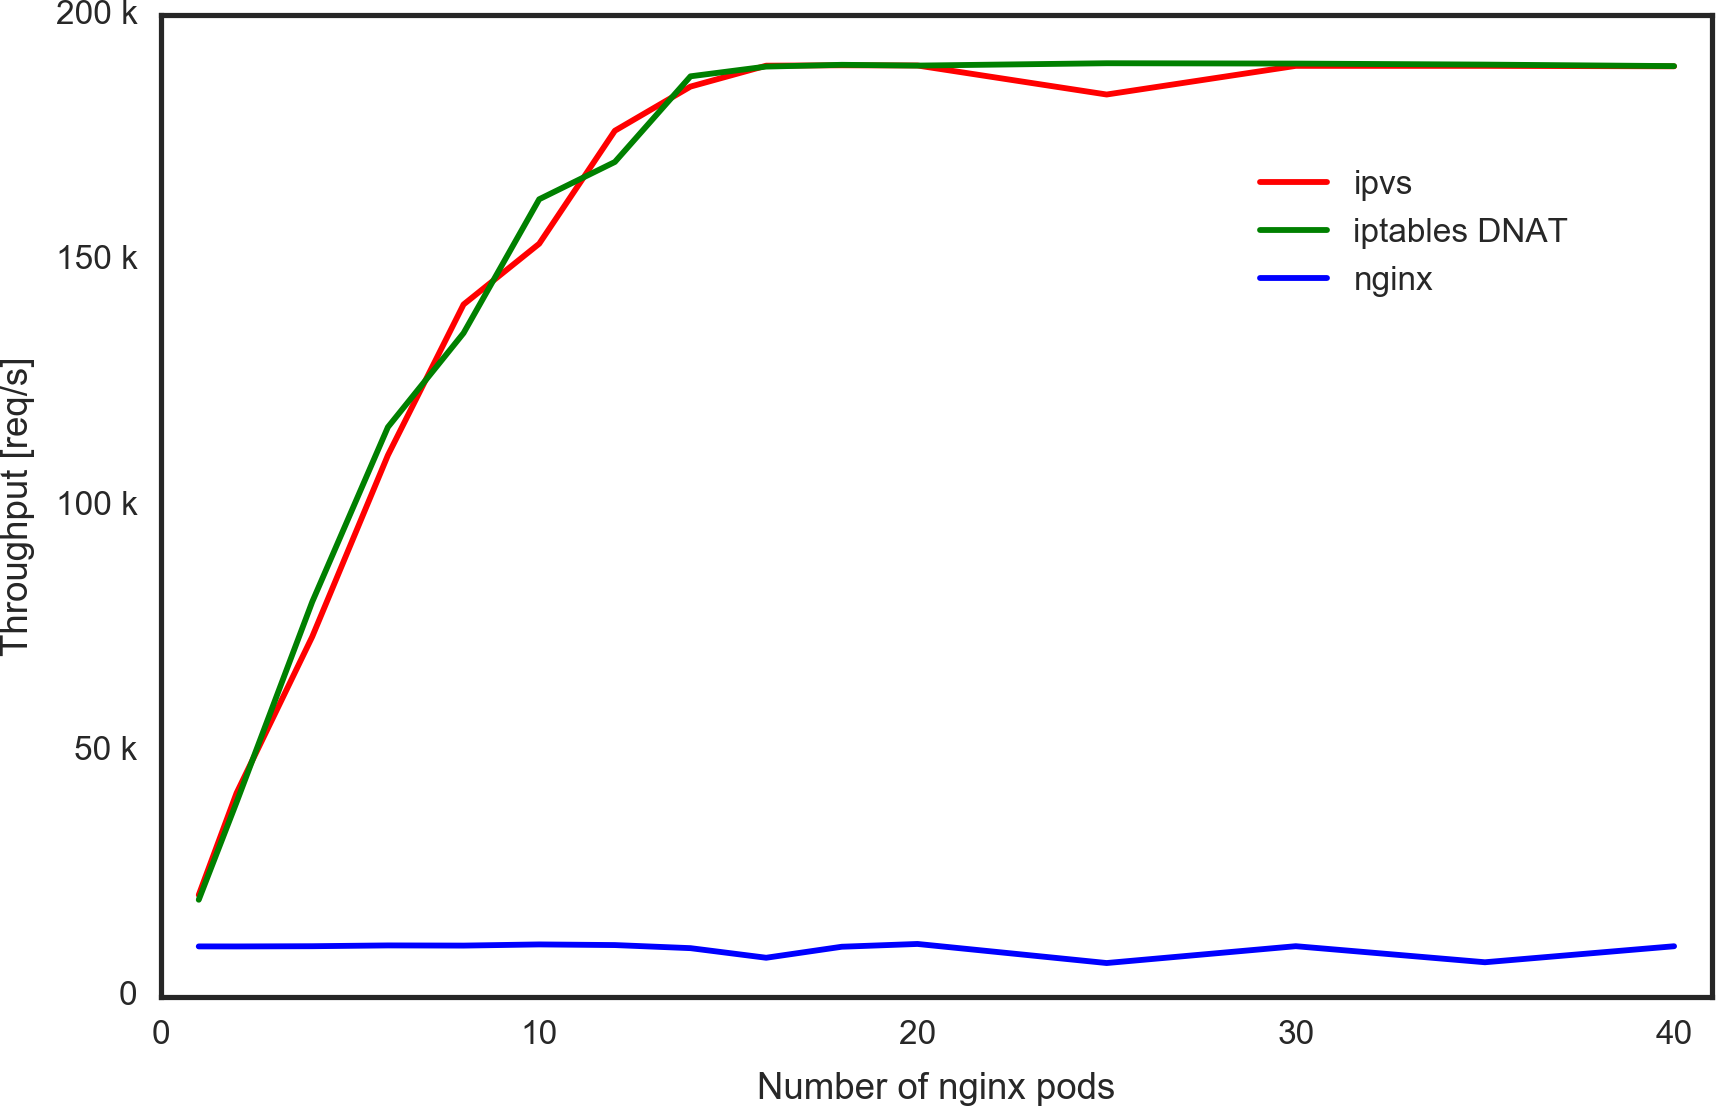
\includegraphics[width=0.75\columnwidth]{Figs/ipvs-iptables-nginx}
  \par\bigskip
  \centering
  \begin{minipage}{0.9\columnwidth}
    \caption[Throughput of ipvs, iptables DNAT and nginx]{
      Throughput of ipvs, iptables DNAT and nginx.
      The performance levels of ipvs and iptables DNAT are almost the same.
      The nginx as a load balancer does not perform well in the experiment.
    }
    \label{fig:ipvs-iptables-nginx}
  \end{minipage}
\end{figure}

\interfootnotelinepenalty=10000

Figure~\ref{fig:ipvs-iptables-nginx} presents the throughput results of the different load balancers.
The performance levels of ipvs, iptables DNAT and nginx as the load balancers are compared.
The throughput of the ipvs and iptables DNAT increases almost linearly with the increasing number of the nginx pods(web servers) from 1 to around 14, and then saturated.
The proposed ipvs load balancer exhibits almost equivalent performance levels as the iptables DNAT as a load balancer.

The saturated throughput indicates the maximum performance level of the load balancer, which could be determined either by network bandwidth between the benchmark client machine and the load balancer node, or CPU performance levels of these machines.
%
In this specific experiment, the performance level was limited by the 1 Gbps bandwidth of the network
\footnote{
All of the nodes use a single interface for communication. 
At the load balancer node, the bandwidth for each direction of Full duplex Ethernet is consumed by the sum of request and response packets.
}, 
which is revealed by packet level analysis using tcpdump\cite{takahashi2018portable}.
%
On average the data size of each request and the corresponding response was about 636 [byte/req] in total, including TCP/IP headers, Ethernet header, and interframe gaps.
Multiplying that with 190K [req/sec] and 8 [bit/byte] will result in 966.72 Mbps.
Therefore the throughput of about 190K [req/sec] is a reasonable number as the maximum performance level in 1Gbps network environment.

While nginx did not show any benefit as the load balancer, the performance of the ipvs load balancer container showed equivalent performance level as iptables DNAT.
This means that the proposed ipvs container load balancer is at least as good as the internal load balancer for Kubernetes in the 1 Gbps network.

\begin{figure}[h]
  \centering
  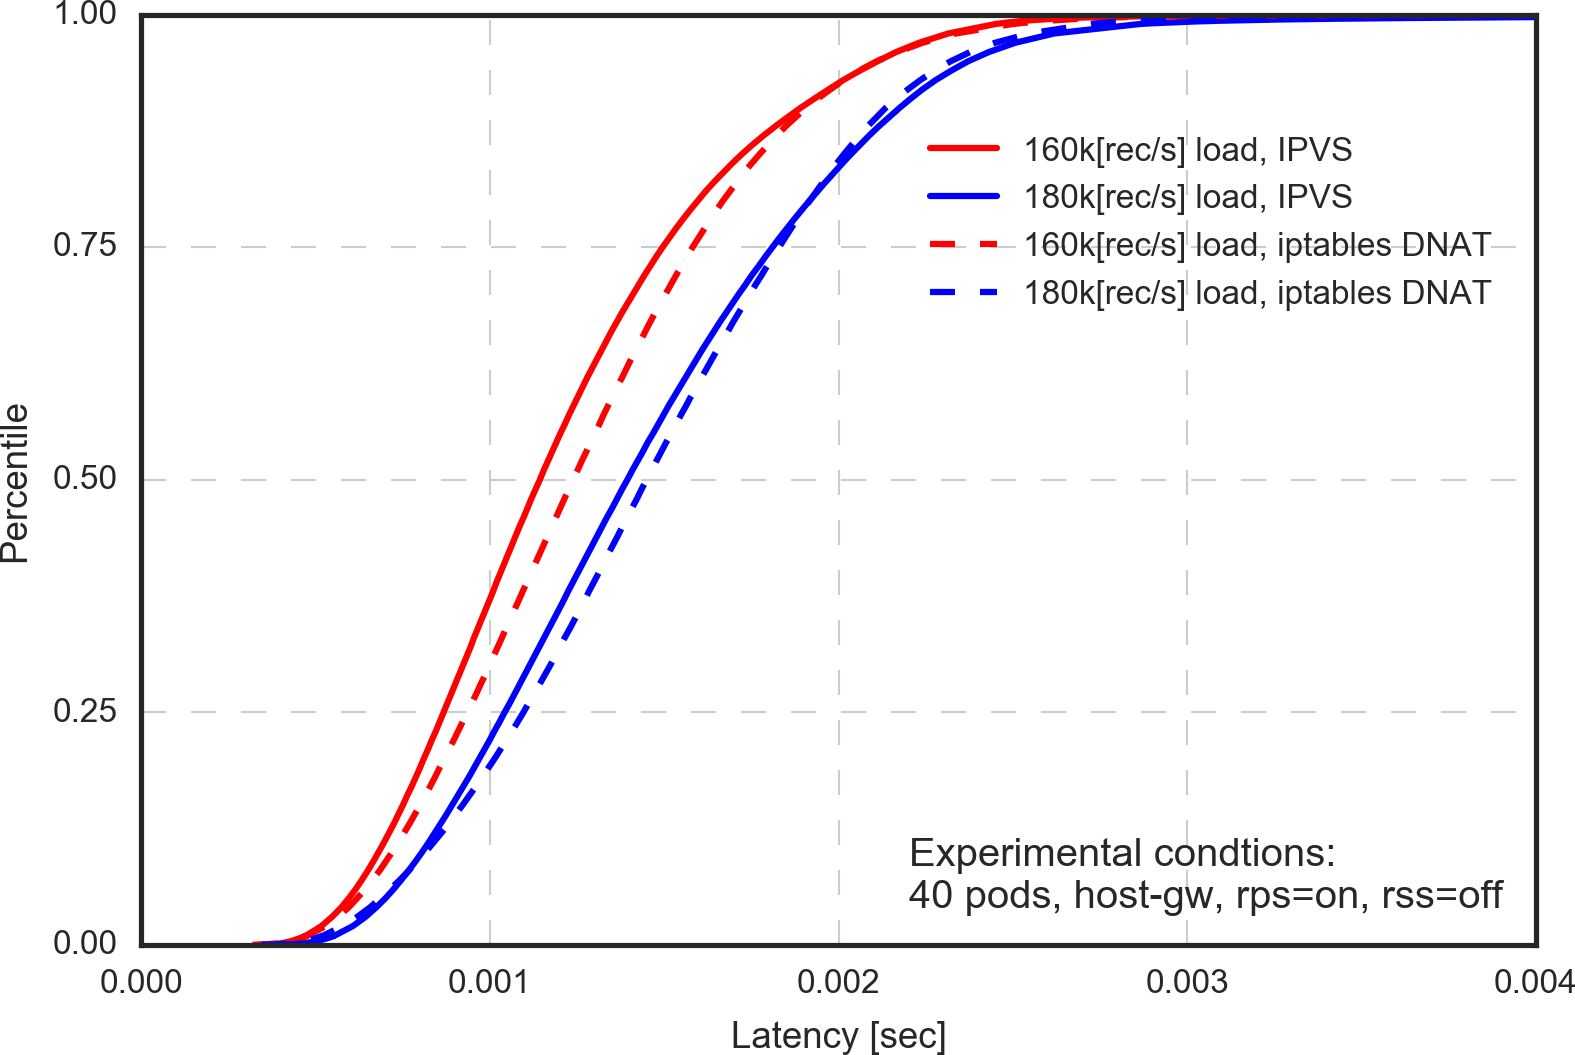
\includegraphics[width=0.75\columnwidth]{Figs/latency_cdf_rps_40pods}
  \par\bigskip
  \centering
  \begin{minipage}{0.9\columnwidth}
    \caption[Latency for ipvs and iptables DNAT]{
      Latency for ipvs and iptables DNAT.
      Cumulative Distribution Function(CDF) of the latency for ipvs and iptables DNAT are compared, at the two constant loads, 160K[req/sec] and 180K[req/sec] .
      Smaller latencies are observed for ipvs.
}
    \label{fig:latency_cdf_rps_40pods}
  \end{minipage}
\end{figure}

Figure~\ref{fig:latency_cdf_rps_40pods} compares Cumulative Distribution Function(CDF) of the load balancer latency at the two constant loads, 160K[req/sec] and 180K[req/sec] for ipvs and iptables DNAT.
It is seen that the latencies are a little bit smaller for ipvs.
For example, the median values at 160K[req/sec] load for ipvs and iptables DNAT are, 1.14 msec and 1.24 msec, respectively.
Also, at 160K[req/sec], they are 1.39 msec and 1.45 msec, respectively.
%
While these may be considered a subtle difference, however, this indicates that proposed load balancer is at least as good as iptables DNAT.

Fig.~\ref{fig:cpu_usage} compares the CPU usage for the proposed ipvs load balancer in container and iptables DNAT at the time of the throughput measurement in the on-premise data center.
Since the CPU usage was higher for the ipvs in a container, the proposed load balancer may be less efficient compared with the iptables DNAT.
However, since single hardware can accommodate 1 Gbps traffic with CPU usage of about 60\%, the authors regard this as a tolerable overhead.

\mytodo[inline]{Change the next sentence depending on the XDP section.}
The authors plan to improve the efficiency of the proposed load balancer by developing a software load balancer using eXpress data path(XDP) technology\cite{hoiland2018express} in the future work and thereby improving the performance levels of the portable load balancer.

\begin{figure}[h]
  \centering
  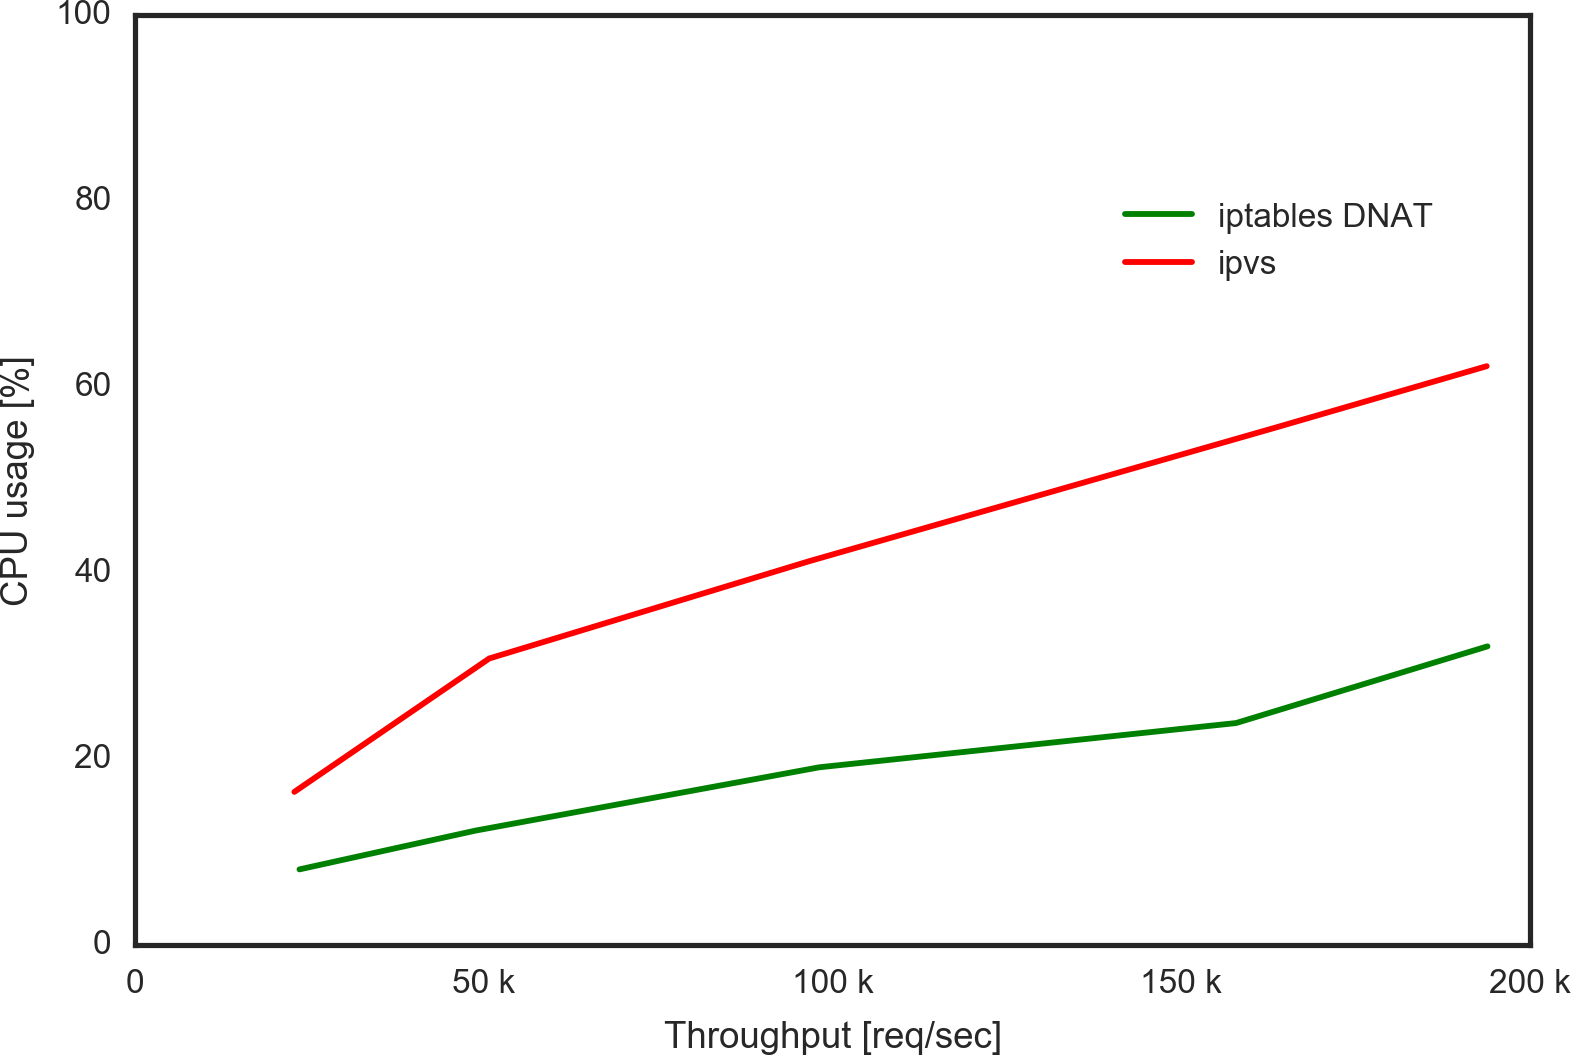
\includegraphics[width=0.75\columnwidth]{Figs/cpu_usage}
  \par\bigskip
  \centering
  \begin{minipage}{0.9\columnwidth}
    \caption[CPU usage of the ipvs and iptables DNAT]{
      CPU usage of the ipvs and iptables DNAT.
      CPU usage of ipvs is higher than that of iptables DNAT.
    }
    \label{fig:cpu_usage}
  \end{minipage}
\end{figure}

\FloatBarrier

\subsubsection{L3DSR using ipvs-tun}

The performance levels of ipvs and iptables DNAT have been limited by 1 Gbps bandwidth.
This can be alleviated in the case of ipvs by using so-called Layer 3 Direct Server Return(L3DSR) setup.
Figure~\ref{fig:benchmark-schem-dsr} shows the schematic diagram illustrating the packet flow of the L3DSR experiment.
The red arrows indicate the route HTTP request packets follow and the blue arrows indicate the route response packets follow.
Since the response packets directly return to the client, the load balance is expected to perform better.

The ipvs has a mode called ipvs-tun.
When the ipvs-tun send out the packets to real servers, it encapsulates the original packet in ipip tunneling packet that is destined to real servers.
The real server receives the packet on a tunl0 device and decapsulates the ipip packet, revealing the original packet.
Since the source IP address of the original packet is maintained, the returning packets are sent directly toward the benchmark client.
In this scheme, the returning packets do not consume the bandwidth nor the CPU power of the load balancer node.
Since iptables DNAT does not have the functions that enable L3DSR settings, this is one of the benefits only available for the ipvs load balancer.

\begin{figure}[h]
  \centering
  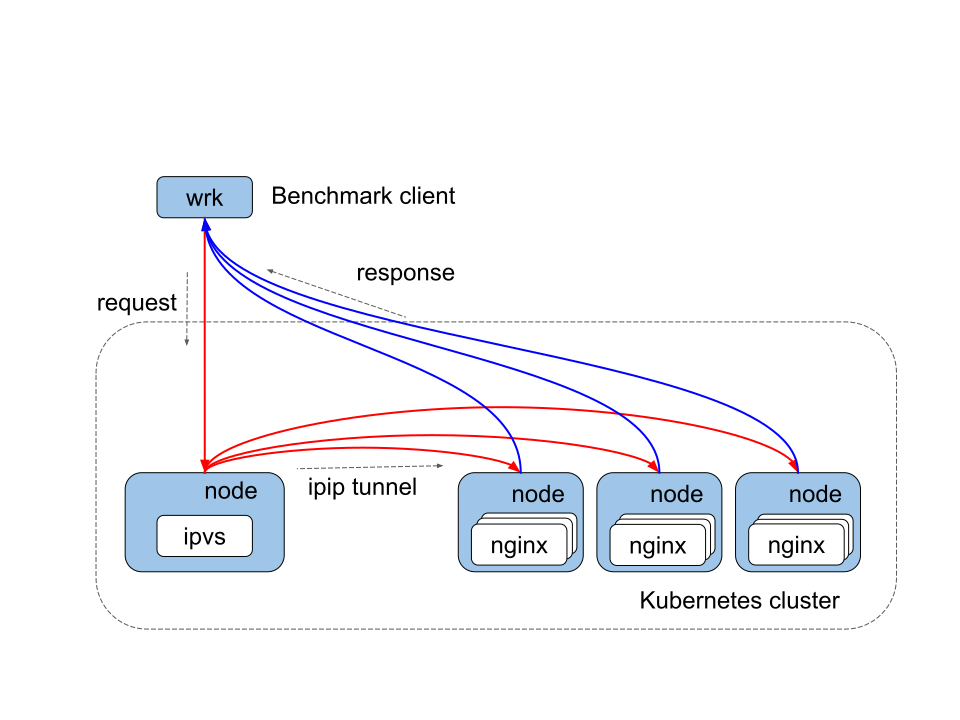
\includegraphics[width=0.8\columnwidth]{Figs/benchmark-schem-dsr}
  \par\bigskip
  \centering
  \begin{minipage}{0.9\columnwidth}
    \caption[Experimental setup for L3DSR throughput measurement]{
      Experimental setup for L3DSR throughput measurement.
      The red arrows indicate the route HTTP request packets follow and the blue arrows indicate the route response packets follow.
      Since the response packets directly return to the client, the load balance is expected to perform better.
    }
    \label{fig:benchmark-schem-dsr}
  \end{minipage}
\end{figure}

\begin{figure}[h]
  \centering
  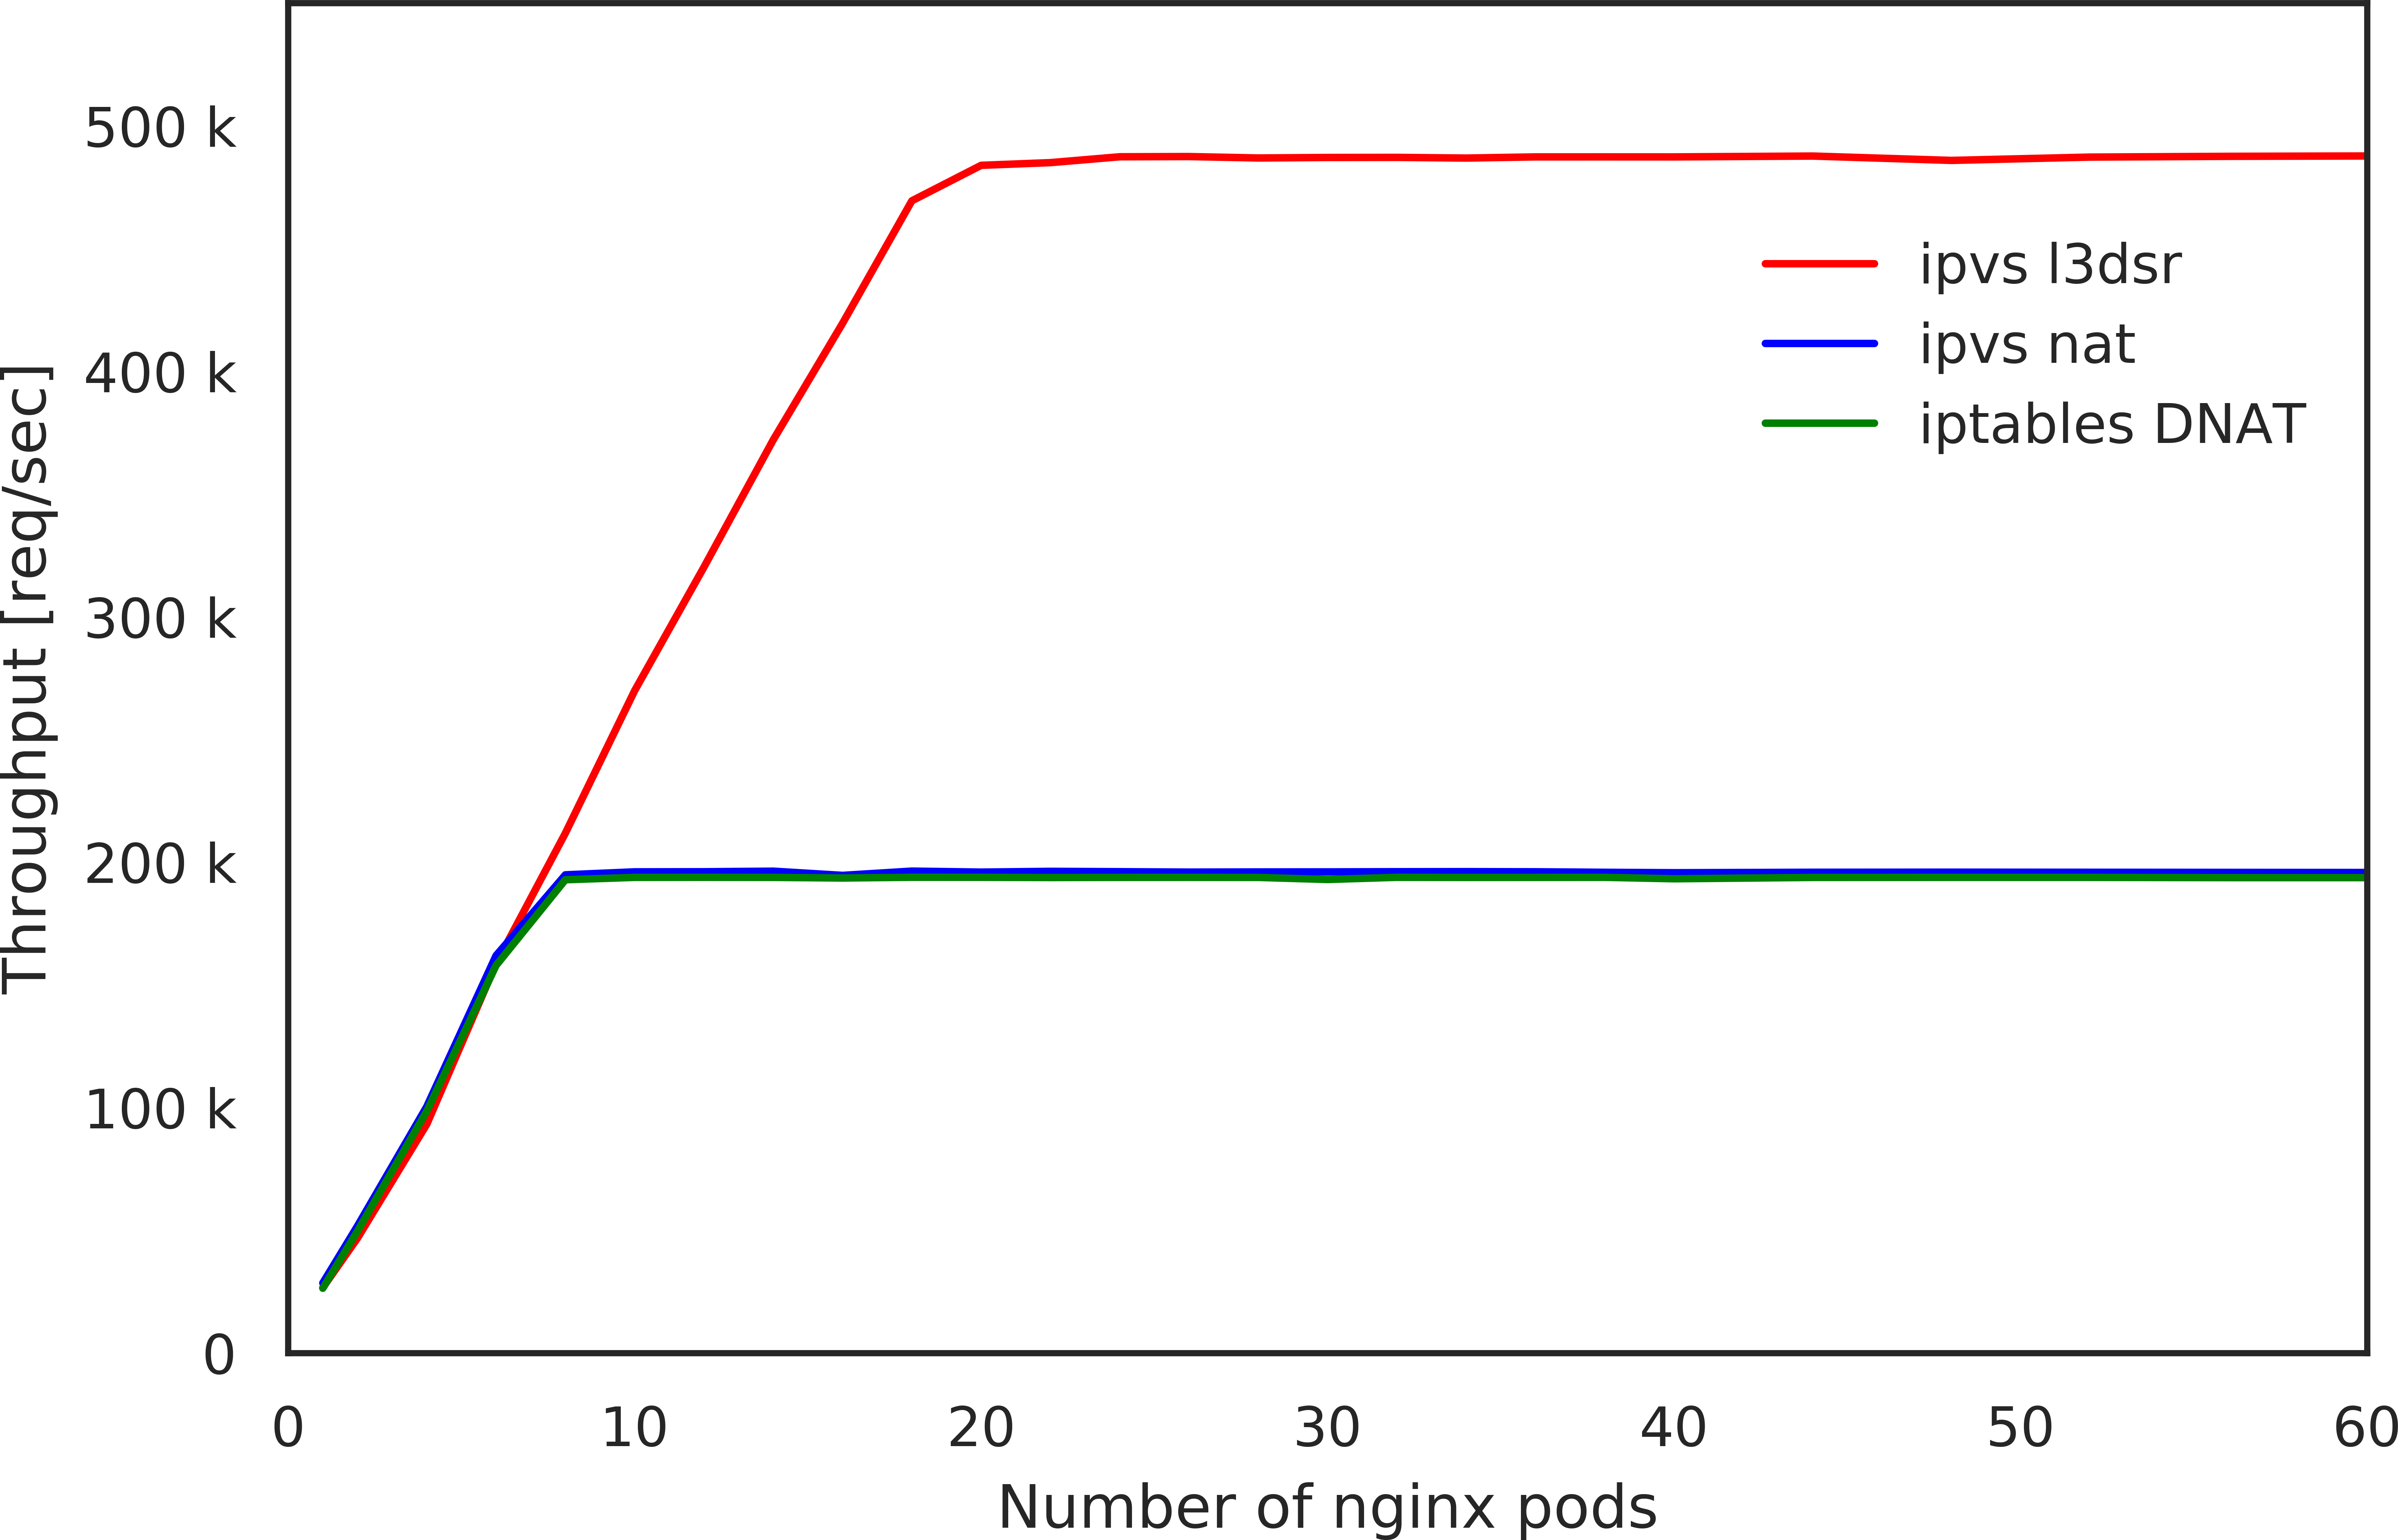
\includegraphics[width=0.75\columnwidth]{Figs/ipvs_l3dsr_1g.png}
  \par\bigskip
  \centering
  \begin{minipage}{0.9\columnwidth}
    \caption[Throughput of L3DSR using ipvs-tun.]{
      Throughput of L3DSR using ipvs-tun.
      The throughput of ipvs-tun is 1.5 times higher than those of conventional ipvs and iptables DNAT.
    }
    \label{fig:ipvs_l3dsr_1g.png}
  \end{minipage}
\end{figure}

The author carried out throughput measurement using the experimental setup shown in Figure~\ref{fig:benchmark-schem-dsr}.
Figure~\ref{fig:ipvs_l3dsr_1g.png} compares the throughput of the ipvs-tun, conventional ipvs and iptables DNAT.
As can be seen in the figure, while the performance levels for ipvs and iptables DNAT exactly match, the performance level of ipvs-tun is much higher than those.
For example, the throughput of ipvs-tun is about 1.5 times higher than those of conventional ipvs and iptables DNAT.
\footnote{The limit is due to the bandwidth of benchmark client's NIC.
Multipling 270K [req/sec] with the response packet size 450[byte/req]\ref{} and 8 [bit/byte] results in 972M [bit/sec] . }

\mytodo[inline]{Add tunneling setup needed on web container for L3DSR, if there is enough time. }

%% The author summarises this section as follows;
%% In experiments in 1Gbps network, the proposed load balancer, i.e., ipvs in container showed equivalent performance level as the iptables DNAT as a load balancer.
%% The efficiency of the ipvs may be inferior to that of iptables DNAT.
%% By using the ipvs-tun (L3DSR mode), the throughput of the proposed load balancer improved 1.5 times.

\FloatBarrier

\section{Cloud experiment}

The throughput measurements were also carried in GCP and AWS to show the containerized ipvs load balancer is runnable even in the cloud environment.
The specifications of virtual machines used for the experiment in both environment are summarized in Table~\ref{fig:gcp_machine_spec} and Table~\ref{fig:aws_machine_spec}.
In the cases of cloud environments, it is easy to change the machine specifications, especially CPU counts.
Therefore, the author measured throughput with several conditions of them.
In the case of GCP, custom instance with 32Gbyte memory and with 8, 16, and 32 CPU are used.
And in the case of AWS instance type of c4.2xlarge, c4.4xlarge, and c4.8xlarge are used.
The vxlan mode of the flannel is used for the overlay network in both of the cloud environment.
As for multicore packet processing, different settings depending on the number of prepared queues for VMs. 
The setting \enquote{(RSS, RPS) = (on, off)} is used in GCP and the setting \enquote{(RSS, RPS) = (off, on)} is used in AWS.

{
\setlength{\tabcolsep}{3em}
\renewcommand{\arraystretch}{1.1}

\begin{table}[h]
  \centering
  \begin{tabular}{ll}
    \hline 
    \multicolumn{2}{l}{[GCP VM Instance Specification for Client and Web Server Nodes ]}   \\
    & Instance type: custom instance \\
    & CPU: Xeon 2.2GHz, 16 cpus \hspace{2cm} \\
    & Memory: 16GB \\
    & NIC: virtio\_net /w 16 rx-queues \\
    & (Node x 6, Client x 1) \\
    & \\
    \multicolumn{2}{l}{[GCP VM Instance Specification for Load balancer Node ]}   \\
    & Instance type: custom instance \\
    & CPU: Xeon 2.2GHz, 8, 16, 32 cpus \hspace{2cm} \\
    & Memory: 16GB \\
    & NIC: virtio\_net /w 8, 16, 32 rx-queues \\
    & (Load balancer x 1) \\
    \hline
  \end{tabular}
  \par\bigskip
  \centering
  \begin{minipage}{0.9\columnwidth}
    \caption[Virtual Machine specifications in GCP experiment]{
Virtual Machine specifications in GCP experiment.
The author measured throughputs using load balancer nodes with 8 CPUs, 16 CPUs, and 32 cups.
The number of rx-queues of each node was 8, 16 and 32, respectively.
Since the same number of rx-queues as the number CPU is prepared, the setting with \enquote{(rss, rps) = (on, off)} is used.
    }
    \label{fig:gcp_machine_spec}
  \end{minipage}
\end{table}
}

{
\setlength{\tabcolsep}{3em}
\renewcommand{\arraystretch}{1.1}

\begin{table}[h]
  \centering
  \begin{tabular}{ll}
    \hline 
    \multicolumn{2}{l}{[AWS VM Instance Specification for Client and Web Server Nodes ]}   \\
    & Instance type: m4.4xlarge \\
    & CPU: Xeon E5-2686 v4 2.30GHz, 16 cpus \\
    & Memory: 64GB \\
    & NIC: ixgbevf /w 2 rx-queues \\
    & (Node x 6, Client x 1) \\
    & \\
    \multicolumn{2}{l}{[AWS VM Instance Specification for Load balancer Node ]}   \\
    & Instance type: c4.2xlarge, c4.4xlarge, c4.8xlarge  \\
    & CPU: Xeon E5-2666 v3 2.90GHz, 8, 16, 36 cpus \\
    & Memory: 15GB, 30GB, 60GB \\
    & NIC: ixgbevf /w 2 rx-queues \\
    & (Load balancer x 1) \\
    \hline
  \end{tabular}
  \par\bigskip
  \centering
  \begin{minipage}{0.9\columnwidth}
    \caption[Virtual Machine specifications in AWS experiment]{
Virtual Machine specifications in AWS experiment.
The author measured throughputs using load balancer nodes with 8 CPUs, 16 CPUs, and 36 CPUs.
Since there are only two rx-queues, the setting with \enquote{(rss, rps) = (off, on)} is used.
    }
    \label{fig:aws_machine_spec}
  \end{minipage}
\end{table}
}


\begin{figure}[h]
  \centering
  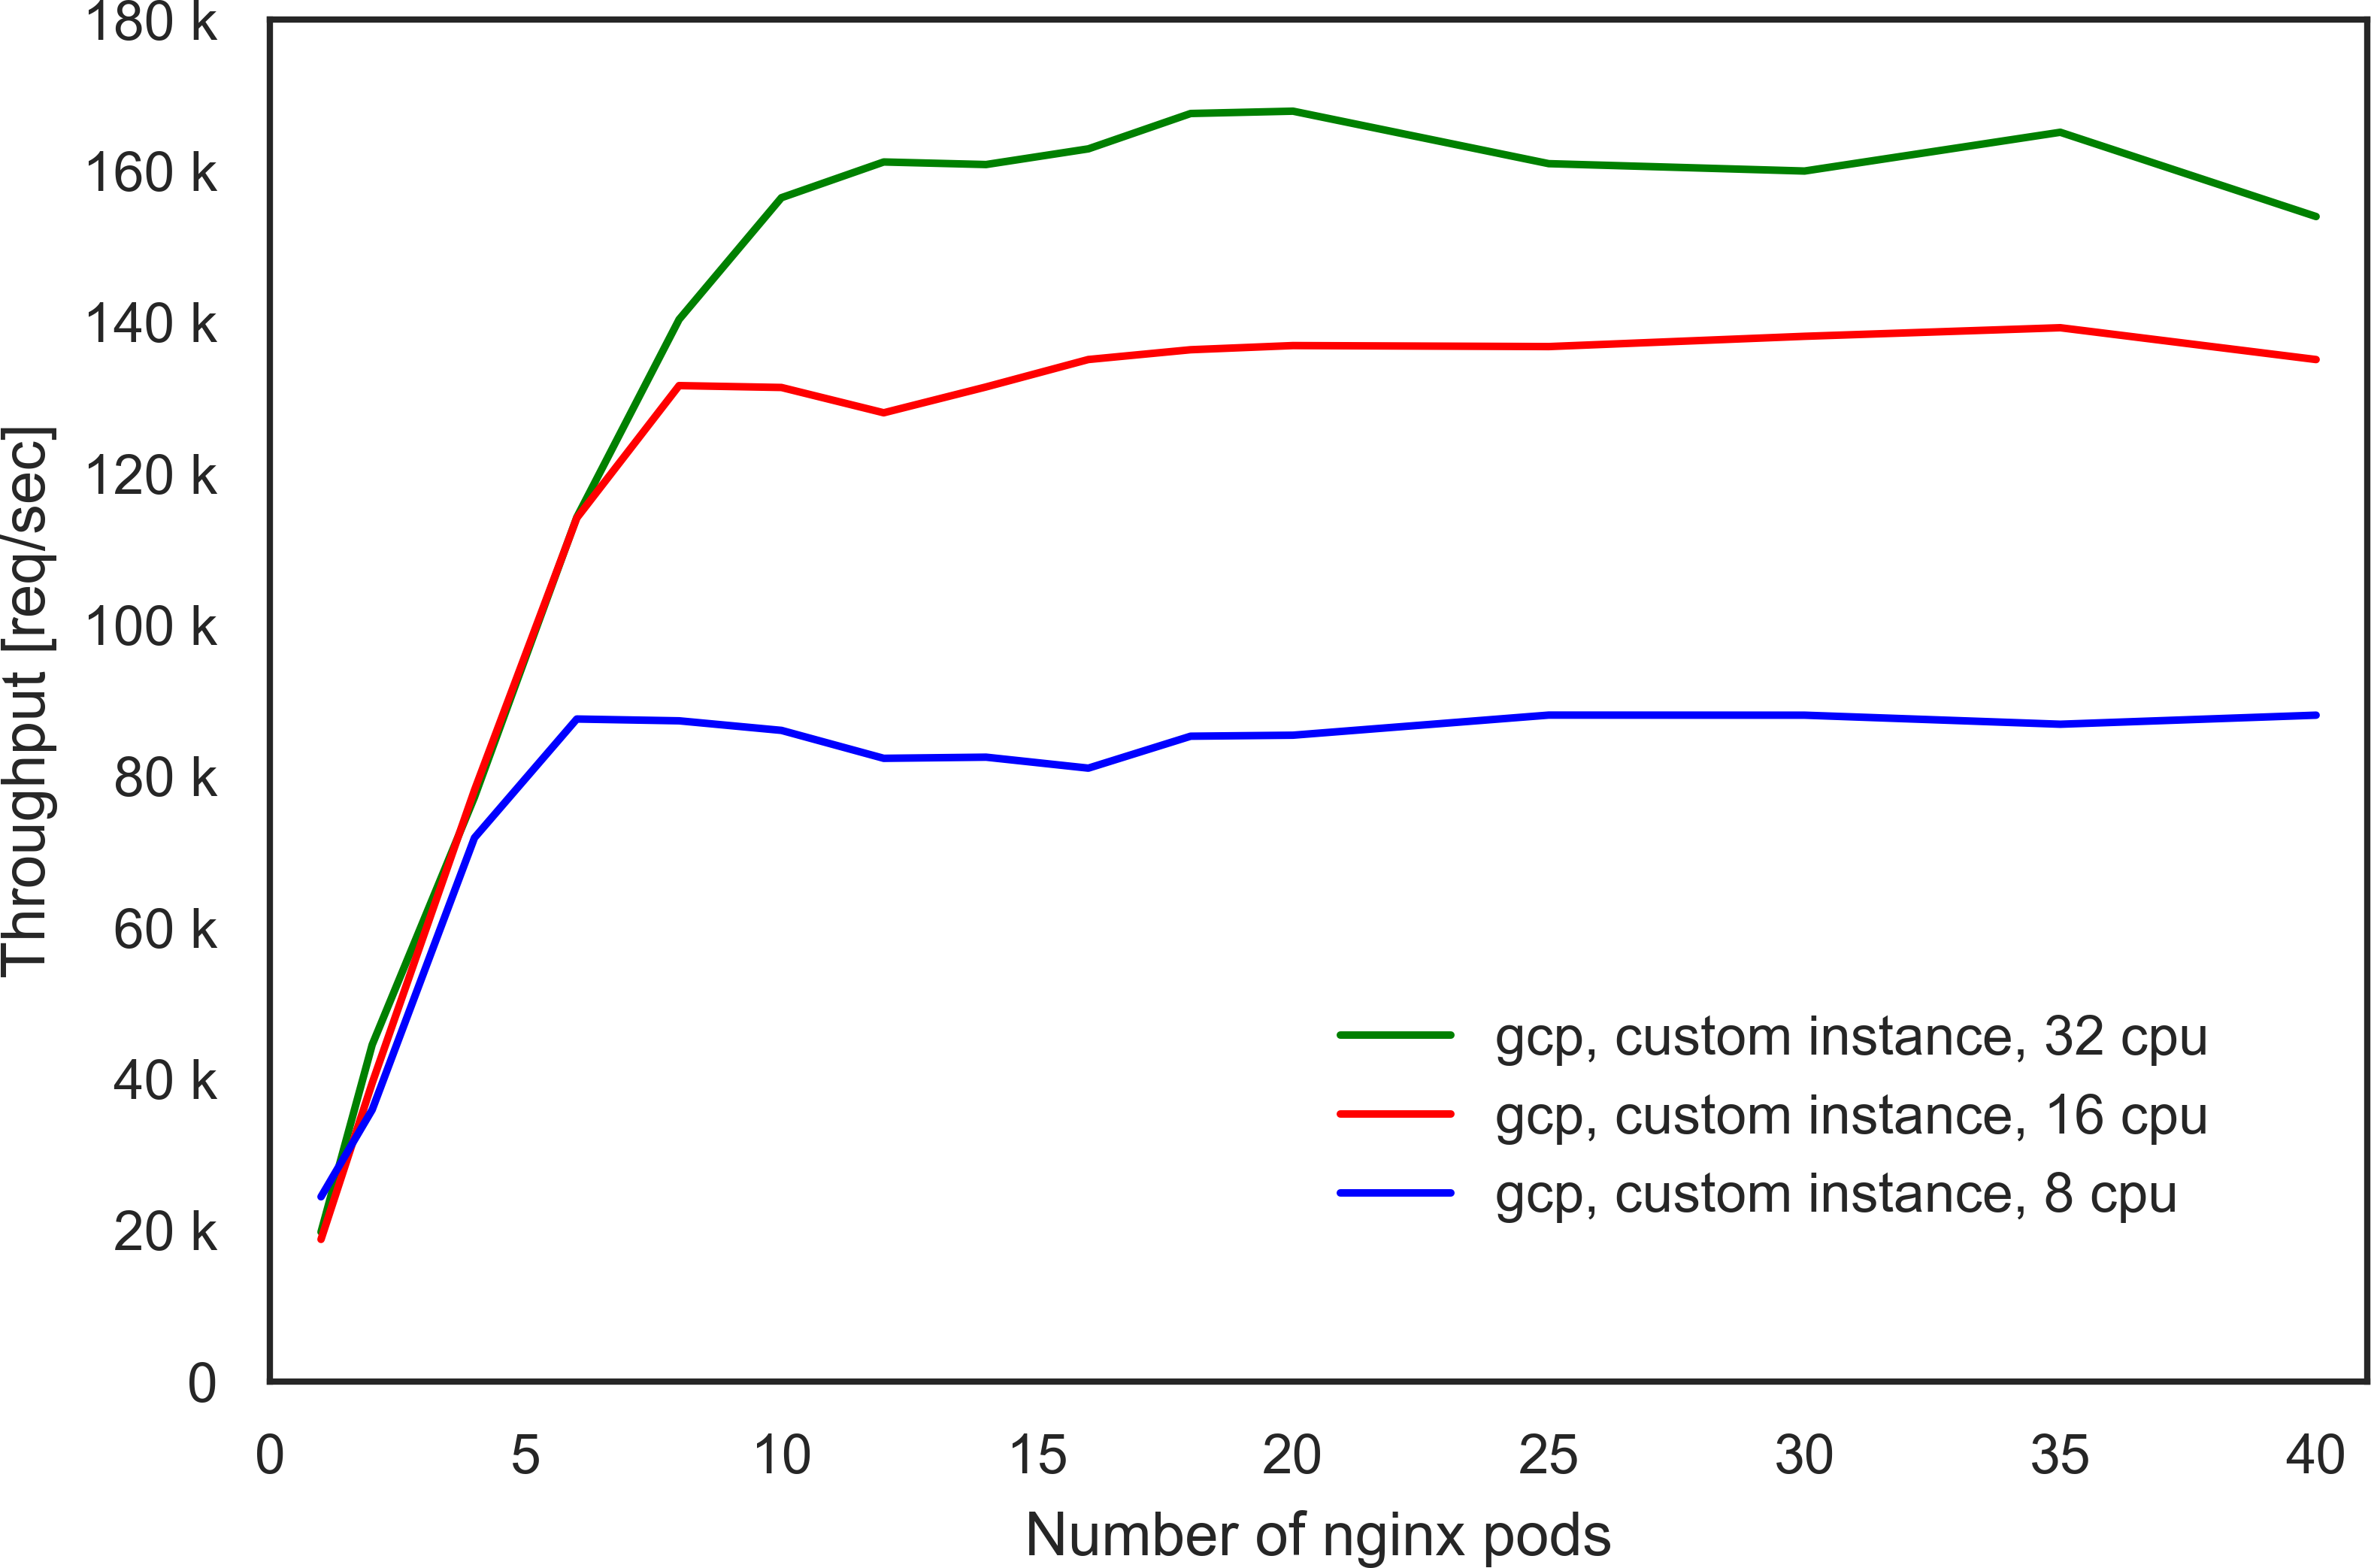
\includegraphics[width=0.75\columnwidth]{Figs/gcp_all_tp}
  \par\bigskip
  \centering
  \begin{minipage}{0.9\columnwidth}
    \caption[Throughput measurement results in GCP]{
Throughput measurement results in GCP.
The throughput increases linearly as the number of nginx {\em pod}s increases until it reaches the saturation level.
The maximum throughput is higher for instances with more virtual CPUs.
    }
    \label{fig:gcp_all_tp}
  \end{minipage}
\end{figure}


\begin{figure}[h]
  \centering
  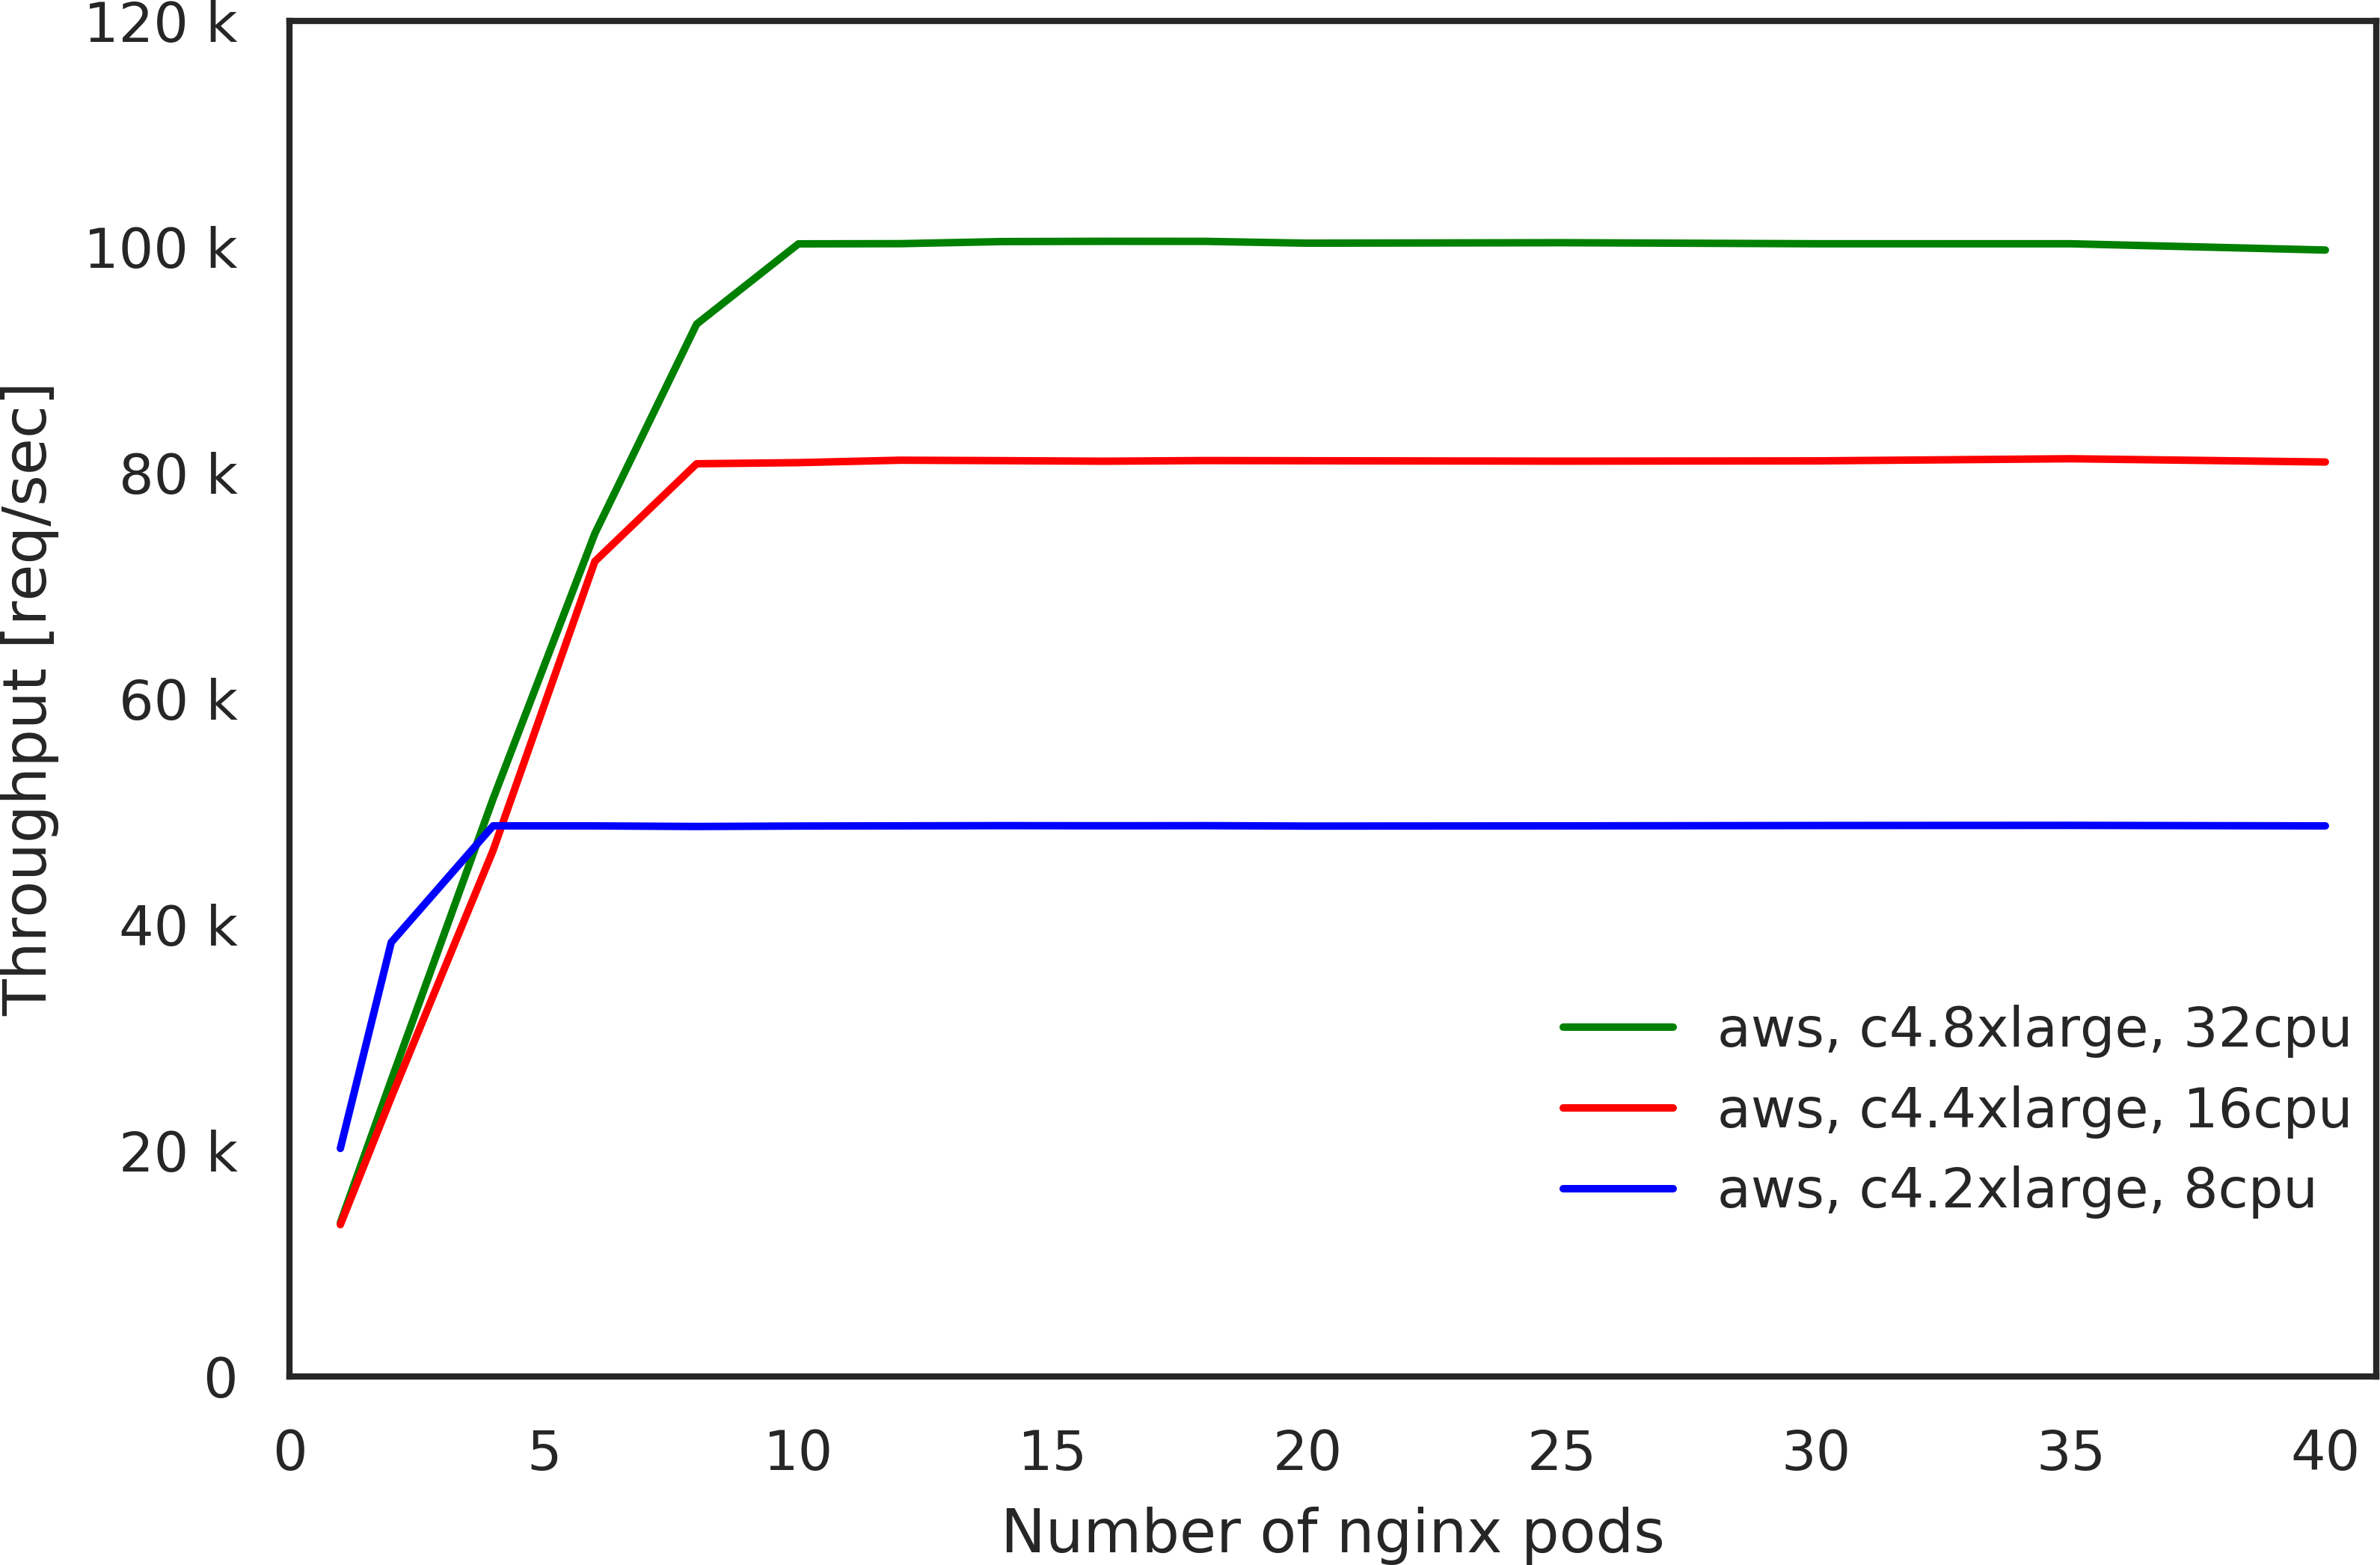
\includegraphics[width=0.75\columnwidth]{Figs/aws_c4_tp}
  \par\bigskip
  \centering
  \begin{minipage}{0.9\columnwidth}
    \caption[Throughput measurement results in AWS]{
Throughput measurement results in AWS.
The throughput increases linearly as the number of nginx {\em pod}s increases until it reaches the saturation level.
The maximum throughput is higher for instances with more virtual CPUs.
    }
    \label{fig:aws_c4_tp}
  \end{minipage}
\end{figure}

Figure~\ref{fig:gcp_all_tp} and Figure~\ref{fig:aws_c4_tp} show the load balancer performance levels that are measured in GCP and AWS, respectively. 
Both results show similar characteristics as the experiment in an on-premise data center in Figure~\ref{fig:ipvs-iptables-nginx}, where throughput increased linearly to a certain saturation level that is determined by either network speed or machine specifications.
It is also seen that the performance levels are higher for load balancer nodes with more CPUs in both GCP and AWS. 
These results indicate that the proposed ipvs load balancers can be run in GCP and AWS, and function properly.

In general, the throughput results in the cloud environments are inferior to those in the on-premise data center, even though much more powerful CPUs are used for VMs in the cloud environment than the experiment in the on-premise data center.
For example, while the maximum throughput of the ipvs load balancer with eight physical cores was ~190K[req/sec] in the on-premise data center(Figure~\ref{fig:ipvs_mcore_proccessing}), the maximum throughput in GCP and AWS are ~160K[req/sec] and ~100K[req/sec], respectively, even with 32 and 36 virtual CPUs.
Although the author suspects that this is probably due to the inefficiency of the virtual machines as opposed to Bare Metal servers,
it is not clear what limits the maximum performance levels of cloud environments. 
The author leaves a detailed analysis for future work.

%% From the first look of the results, since changing CPU counts changed the load balancer's throughput saturation levels, we thought VM's computation power limited the performance levels.
%% However, since there are cases in the cloud environment, where changing the VM types or CPU counts also changes the network bandwidth limit, a detailed analysis is further required in the future to clarify which factor limits the throughput in the cases of these cloud environments.
%% Still, we can say that 

\mytodo[inline]{Mention that BGP peering is unavailable in cloud , in somewhere.}

\FloatBarrier

\section{Redundancy with ECMP}

While containerizing ipvs makes it runnable in any environment, it is essential to discuss how to route the traffic to the ipvs container in a redundant and scalable manner.
The ECMP technique is expected to make the load balancers redundant and scalable since all the load balancer containers act as active.
The author examined the behavior of the ECMP routing table updates, by changing the number of the load balancers.
After that, in order to explore the scalability, the author also measured the throughput from a benchmark client with ECMP routes when multiple of the ipvs container load balancers are deployed.

\begin{figure}[h]
  \centering
  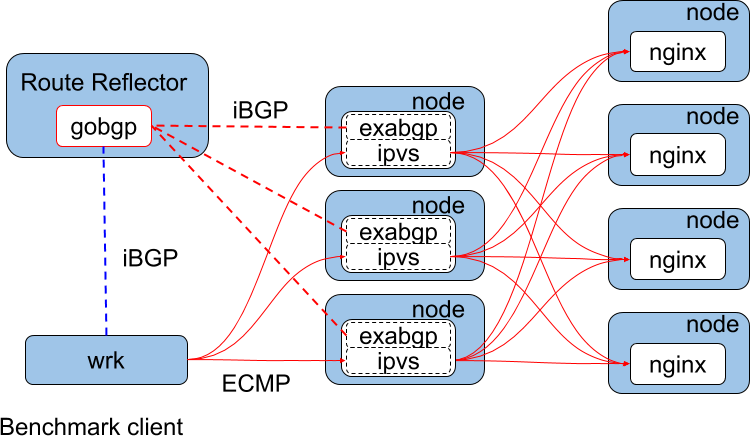
\includegraphics[width=0.9\columnwidth]{Figs/lb_ecmp_schem}

  \par\bigskip
  \centering
  \begin{minipage}{0.9\columnwidth}
    \caption[Benchmark setup for ECMP experiment]{
      Benchmark setup for ECMP experiment.
      Each load balancer pods consists of both an ipvs container and an exabgp container.
      The routing table of the benchmark client is updated by BGP protocol through a route reflector.
    }
    \label{fig:ecmp-benchmark-schem}
  \end{minipage}
\end{figure}

{
\setlength{\tabcolsep}{1em}
\renewcommand{\arraystretch}{1.2}

\begin{table}[h]
  \centering
  \begin{tabular}{ll}
    \hline 
    \multicolumn{2}{l}{[Hardware Specification]}   \\
    & CPU: Xeon E5-2450 2.10GHz x 8 (with Hyper Threading) \\
    & Memory: 32GB \\
    & NIC: Broadcom BCM5720 with 4 rx-queues, 1 Gbps \\
    & (Node x 6, Load Balancer x 4) \\
    & \\
    & CPU: Xeon E5-2450 2.10GHz x 8 (with Hyper Threading) \\
    & Memory: 32GB \\
    & NIC: Intel X550 \\
    & (Client x 1) \\
    & \\
    \multicolumn{2}{l}{[Node Software]}  \\
    & OS: Debian 9.5, linux-4.16.8 \\
    & Kubernetes v1.5.2 \\
    & flannel v0.7.0 \\
    & etcd version: 3.0.15 \\
    & \\
    \multicolumn{2}{l}{[Container Software]}   \\
    & Keepalived: v1.3.2 (12/03,2016) \\
    & nginx : 1.15.4(web server) \\
    & \\
    \multicolumn{2}{l}{[BGP Software]}   \\
    & gobgp version 1.33 (route reflector \& benchmark client) \\
    & exabgp 3.4.17 (load balancer) \\
  \hline 
  \end{tabular}
  \par\bigskip
  \centering
  \begin{minipage}{0.9\columnwidth}
    \caption[Hardware and software specifications for ECMP experiment]{
      Hardware and software specifications for ECMP experiment.
      The NIC of the benchmark client is 10 Gbps card to measure the aggregated throughput of 1Gbps load balancers.
    }
    \label{tab:ecmp-hw_sw_spec}
  \end{minipage}
\end{table}
}

Figure~\ref{fig:ecmp-benchmark-schem} shows the schematic diagram of the experimental setup. Table~\ref{tab:ecmp-hw_sw_spec} summarizes hardware and software specifications.
Notable differences from the previous throughput experiment in Figure~\ref{fig:benchmark-schem} and Table~\ref{tab:hw_machine_spec} are as follows;
1) Each load balancer pods now consists of both an ipvs container and an exabgp container.
2) The routing table of the benchmark client is updated by BGP protocol through a route reflector.
3) The NIC of the benchmark client has been changed to 10 Gbps card since now we have multiple of ipvs container load balancers that are capable of filling up 1 Gbps bandwidth.
4) Some of the software have been updated to the most recent versions at the time of the experiment.

\FloatBarrier

{
\setlength{\tabcolsep}{1em}
\renewcommand{\arraystretch}{1.2}

\begin{table}[h]

  \begin{subtable}{.9\textwidth}
    \centering
    \begin{tabular}{l}
    \hline 
    10.1.1.0/24 via 10.0.0.106 dev eth0 proto zebra metric 20 \\
    \hline
    \end{tabular}
    \caption{With single load balancer {\em pod}.}
    \label{tab:single}
  \end{subtable}

  \par\bigskip

  \begin{subtable}{.9\textwidth}
    \centering
    \begin{tabular}{ll}
      \hline
      \multicolumn{2}{l}{10.1.1.0/24 proto zebra metric 20 } \\
      \hspace{15 mm}
      & nexthop via 10.0.0.105  dev eth0 weight 1 \\
      & nexthop via 10.0.0.106  dev eth0 weight 1 \\
      & nexthop via 10.0.0.107  dev eth0 weight 1 \\
      \hline
    \end{tabular}
    \caption{With three load balancer {\em pod}s.}
    \label{tab:three}
  \end{subtable}
  
  \par\bigskip
  
  \begin{subtable}{.9\textwidth}
    \centering
    \begin{tabular}{ll}
      \hline
      \multicolumn{2}{l}{10.1.1.0/24 pro to zebra metric 20 } \\
      \hspace{15 mm}
      & nexthop via 10.0.0.107  dev eth0 weight 1 \\
      & nexthop via 10.0.0.105  dev eth0 weight 1 \\
      & nexthop via 10.0.0.106  dev eth0 weight 1 \\
      \multicolumn{2}{l}{10.1.2.0/24 proto zebra metric 20 } \\
      \hspace{15 mm}
      & nexthop via 10.0.0.107  dev eth0 weight 1 \\
      & nexthop via 10.0.0.106  dev eth0 weight 1 \\
      \hline
    \end{tabular}
    \caption{For a service with three load balancer {\em pod}s and a service with two load balancer {\em pod}s.}
    \label{tab:double_svc}
  \end{subtable}
  
  \par\bigskip
  \centering
  \begin{minipage}{0.9\columnwidth}
    \caption[ECMP routing tables]{
ECMP routing tables. All the routing rules are updated by zebra.
(a) According to this entry, packets toward 10.1.1.0/24 are forwarded to 10.0.0.106.
(b) There is a routing rule with three next hops towards 10.1.1.0/24, each of which is the node where the load balancer pods are running.
The weights of the three next-hops are all 1.
(c) There are two routing rules regarding the services with different service IPs, one with three load balancers and the other with two load balancers.
These load balancers share the same group of nodes, i.e., (10.0.0.105,10.0.0.106,10.0.0.107).
    }
    \label{tab:exabgp_routing_table}
  \end{minipage}
\end{table}
}

First, the author examined ECMP functionality by monitoring the routing table on the benchmark client.
Table~\ref{tab:exabgp_routing_table}~(\subref{tab:single}) shows the routing table entry on the router when a single load balancer pod exists.
From this entry, it is seen that packets toward 10.1.1.0/24 are forwarded to 10.0.0.106 where the load balancer pod is running.
It also shows that this routing rule is updated by zebra.

The routing table entry in Table~\ref{tab:exabgp_routing_table}~(\subref{tab:three}) is seen when the number of the load balancer pods is increased to three.
There are three next hops towards 10.1.1.0/24, each of which is the node where the load balancer pods are running.
The weights of the three next-hops are all 1.
The update of the routing entry was almost instant as the author increased the number of the load balancers.

Table~\ref{tab:exabgp_routing_table}~(\subref{tab:double_svc}) shows the case where the author additionally started new service with two load balancer pods with service addresses in 10.1.2.0/24 range.
It was possible to accommodate two services with different service IPs on the same group of nodes(10.0.0.105, 10.0.0.106, 10.0.0.107). 
The one has three load balancers and the other has two load balancers.
The update of the routing entry was almost instant as the author started the load balancers for the second service.

As far as the route withdrawal is concerned, if an exabgp is killed by SIGKILL or SIGTERM the kernel of the node close the BGP connection by sending out a packet with FIN flag to the peer gobgpd on the route reflector, and thus the route is withdrawn immediately.
The gobgp on the route reflector also periodically check the BGP connection, and if the peer exabgp container is unresponsive for more than the specified duration, “hold-time“ setting in gobgpd, it will also terminate the connection and withdraw the route.
The packets arriving within that duration will be dropped.
However, it is possible to set up the “hold-time” short enough so that the retransmitted TCP packets from the client will be forwarded correctly to functioning load balancers.

\FloatBarrier

\begin{figure}[h]
  \centering
  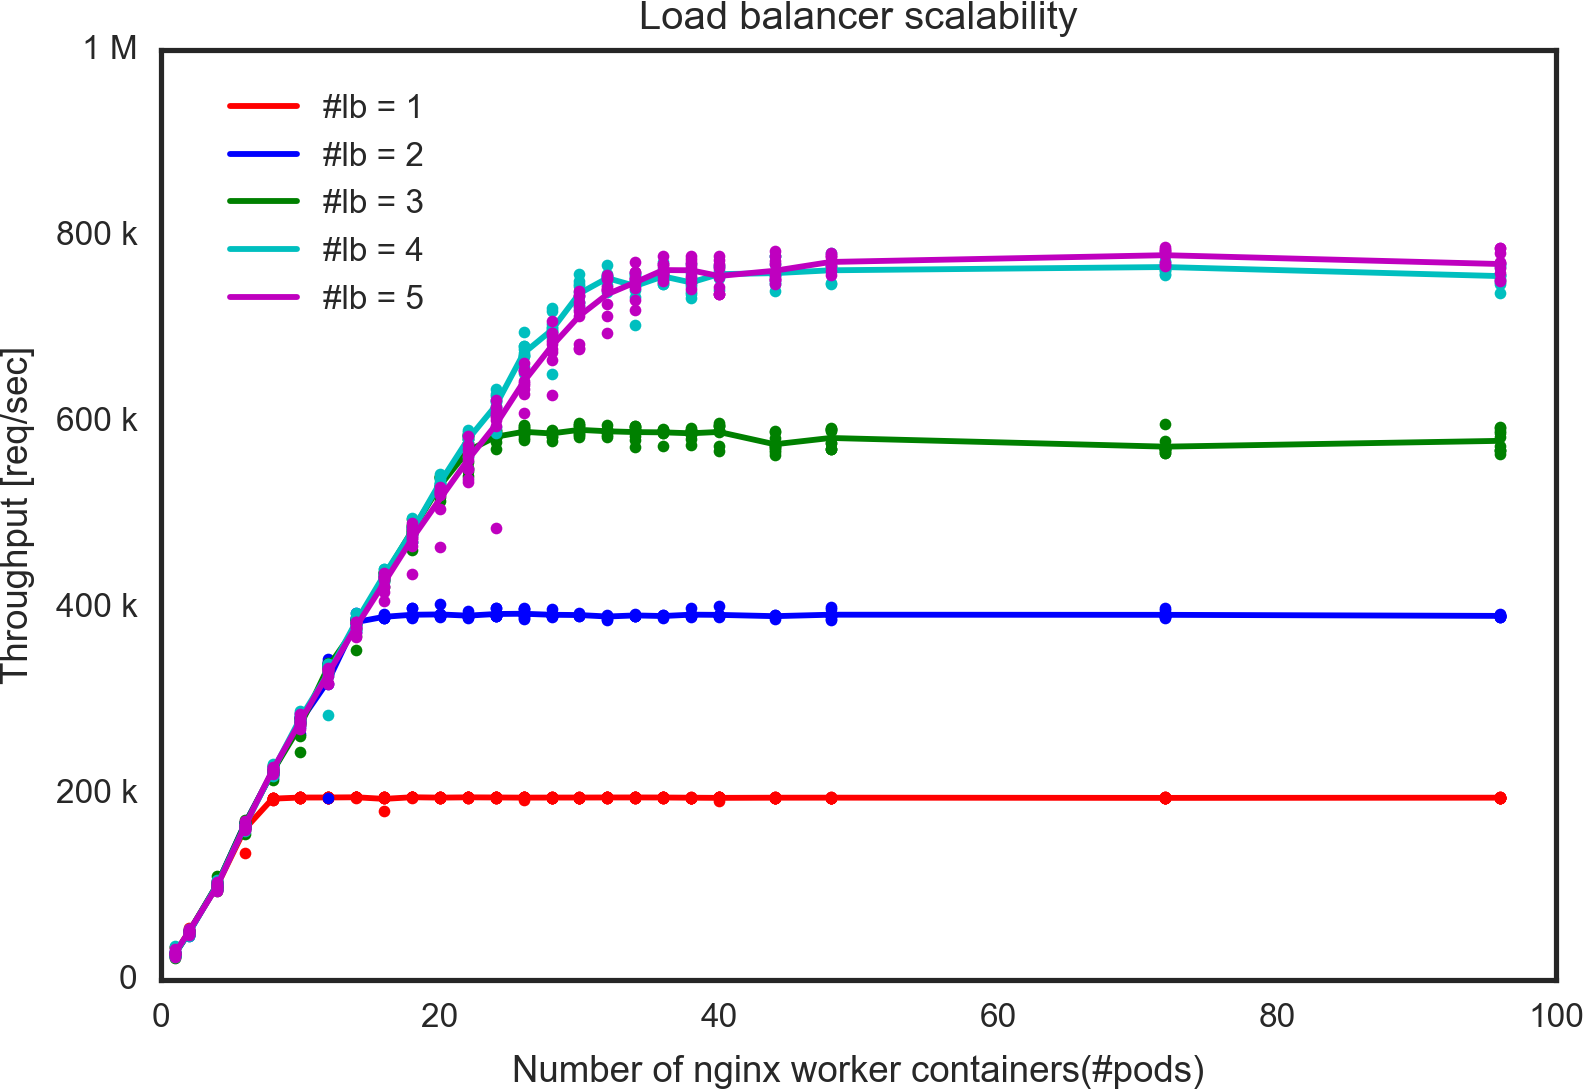
\includegraphics[width=0.9\columnwidth]{Figs/ecmp_lb_cubic}
  \par\bigskip
  \centering
  \begin{minipage}{0.9\columnwidth}
    \caption[Throughput of ECMP redundant load balancer]{
      Throughput of ECMP redundant load balancer.
      The throughputs are measured for a single load balancer(lb x1), two(lb x2), three(lb x3) and four(lb x4) load balancers.
    }
    \label{fig:ecmp_lb_cubic}
  \end{minipage}
\end{figure}

\begin{figure}[h]
  \centering
  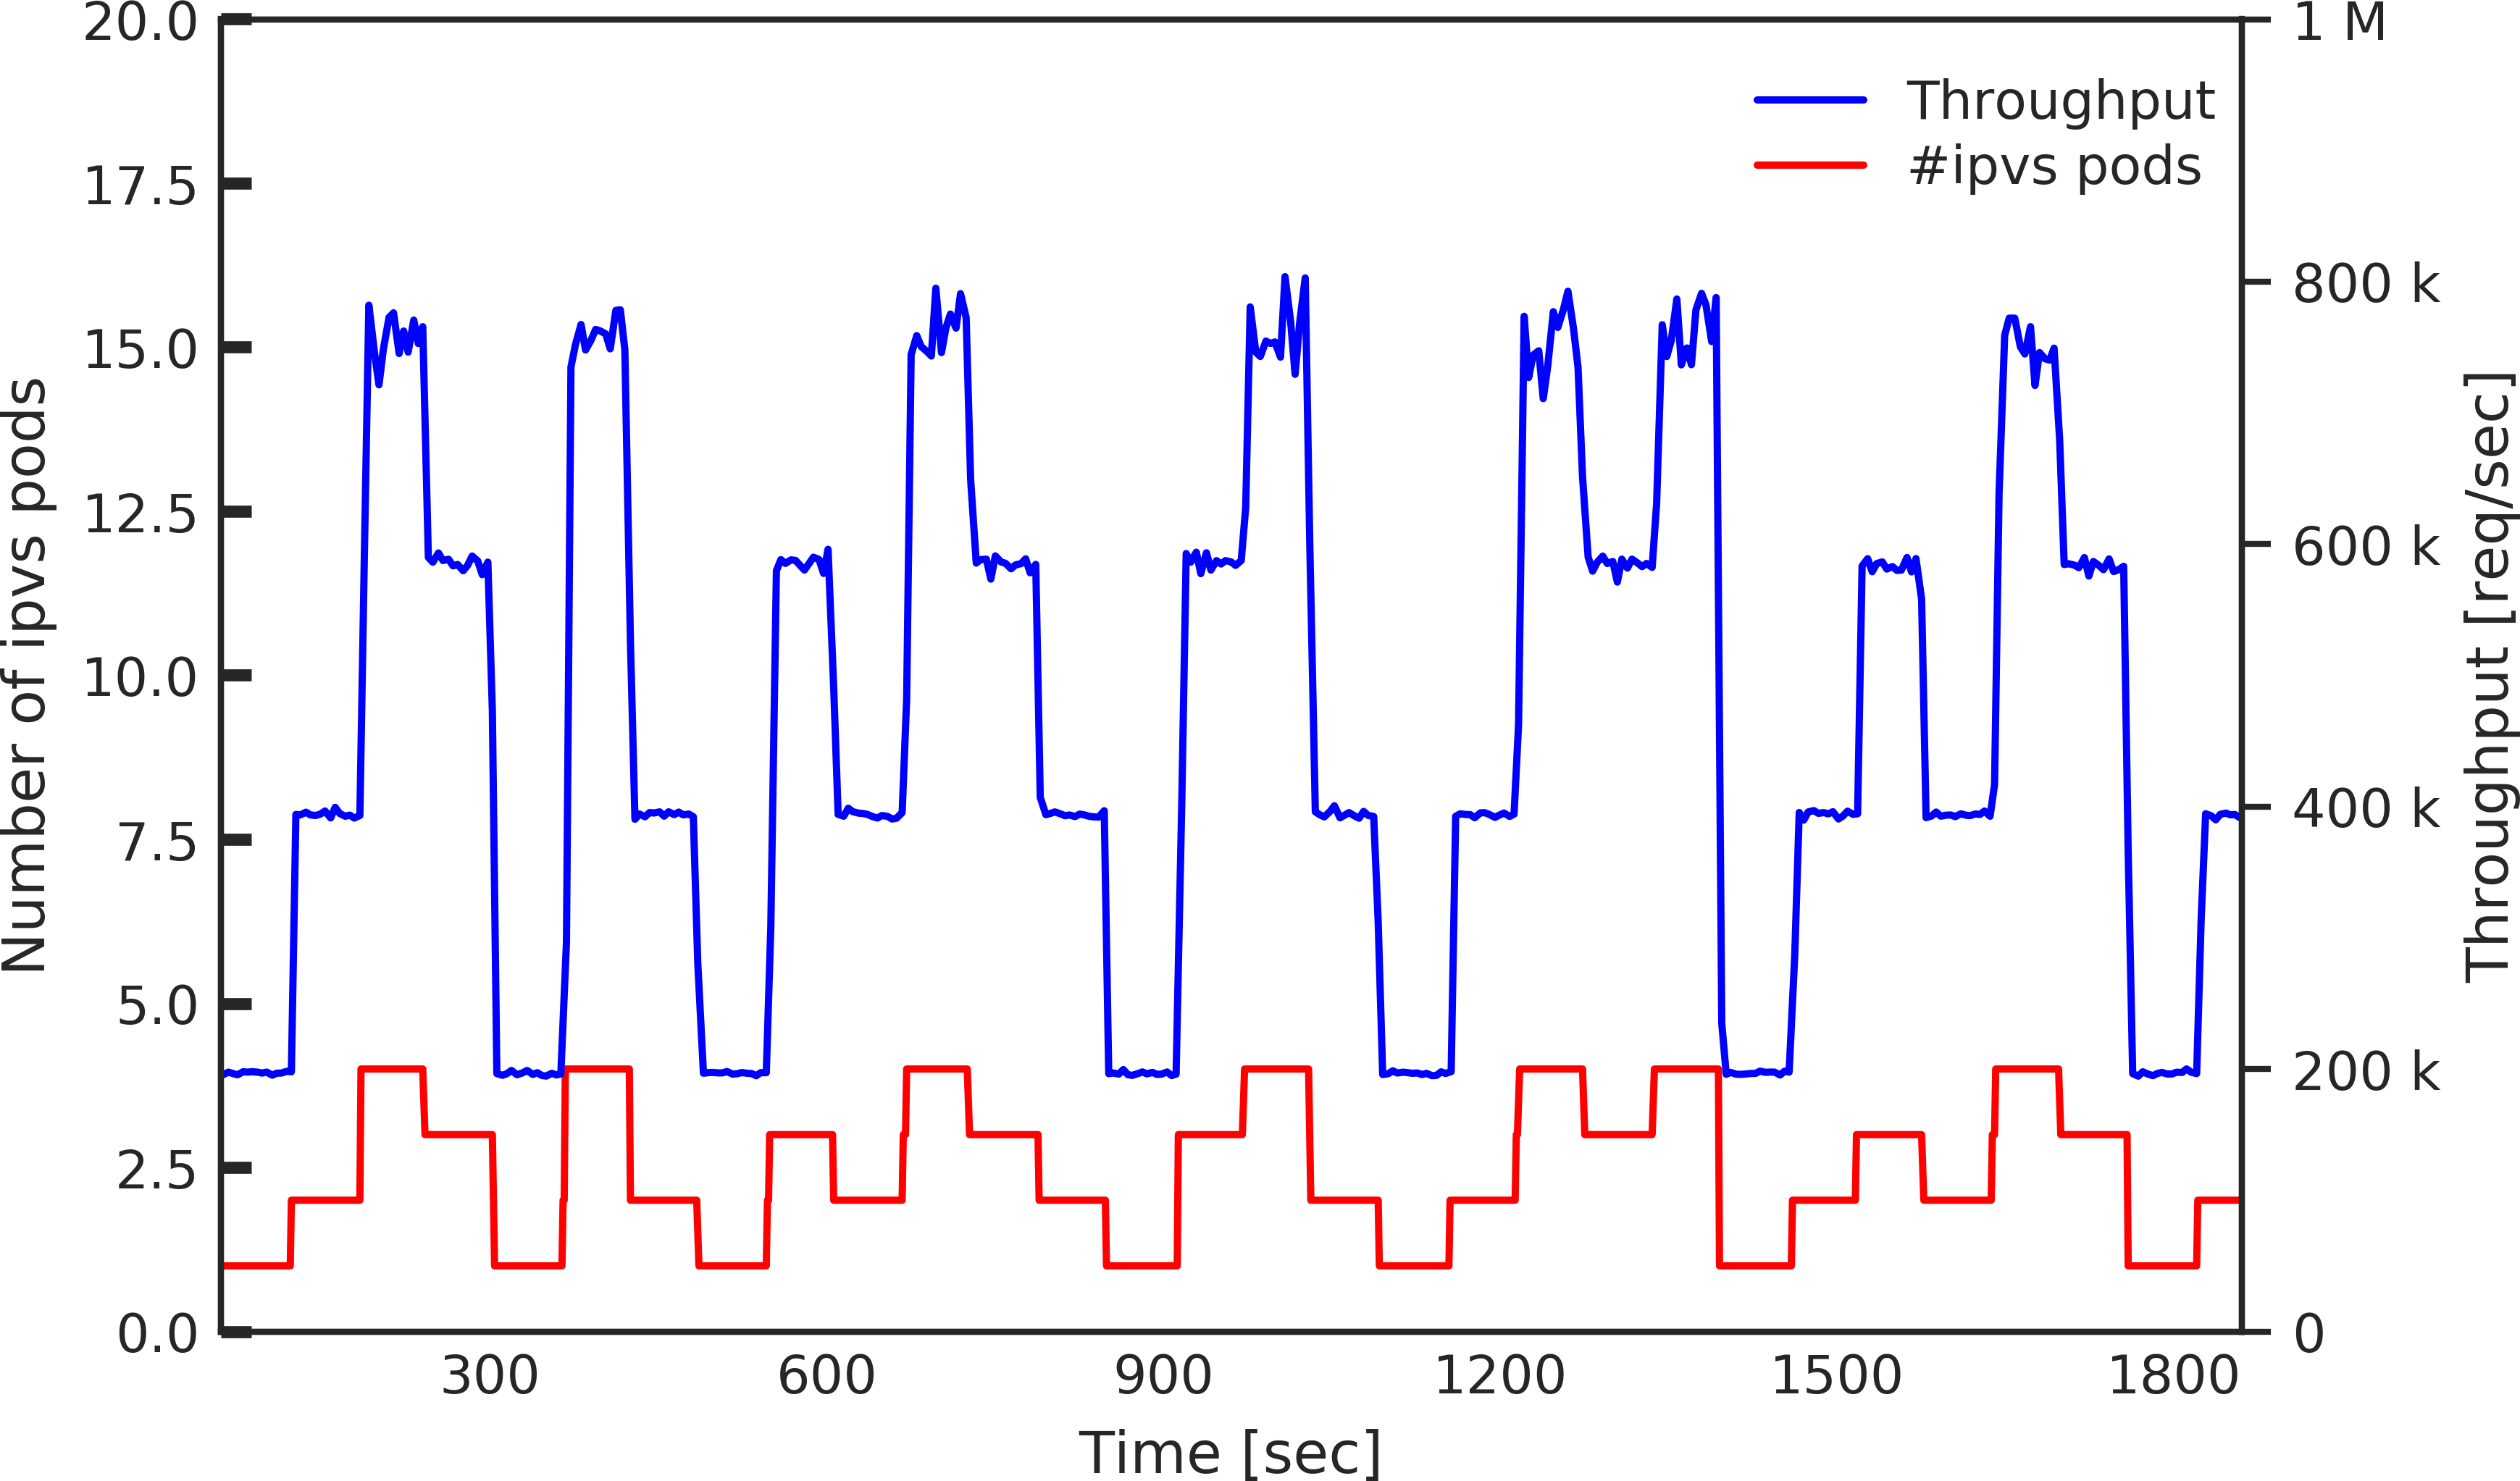
\includegraphics[width=0.9\columnwidth]{Figs/ecmp_response}
  \par\bigskip
  \centering
  \begin{minipage}{0.9\columnwidth}
    \caption[Throughput responsiveness]{
      Throughput responsiveness.
      Throughput responsiveness when the number of load balancers is changed randomly in every 60 seconds is shown.
    }
    \label{fig:ecmp_response}
  \end{minipage}
\end{figure}


\begin{figure}[h]
  \centering
  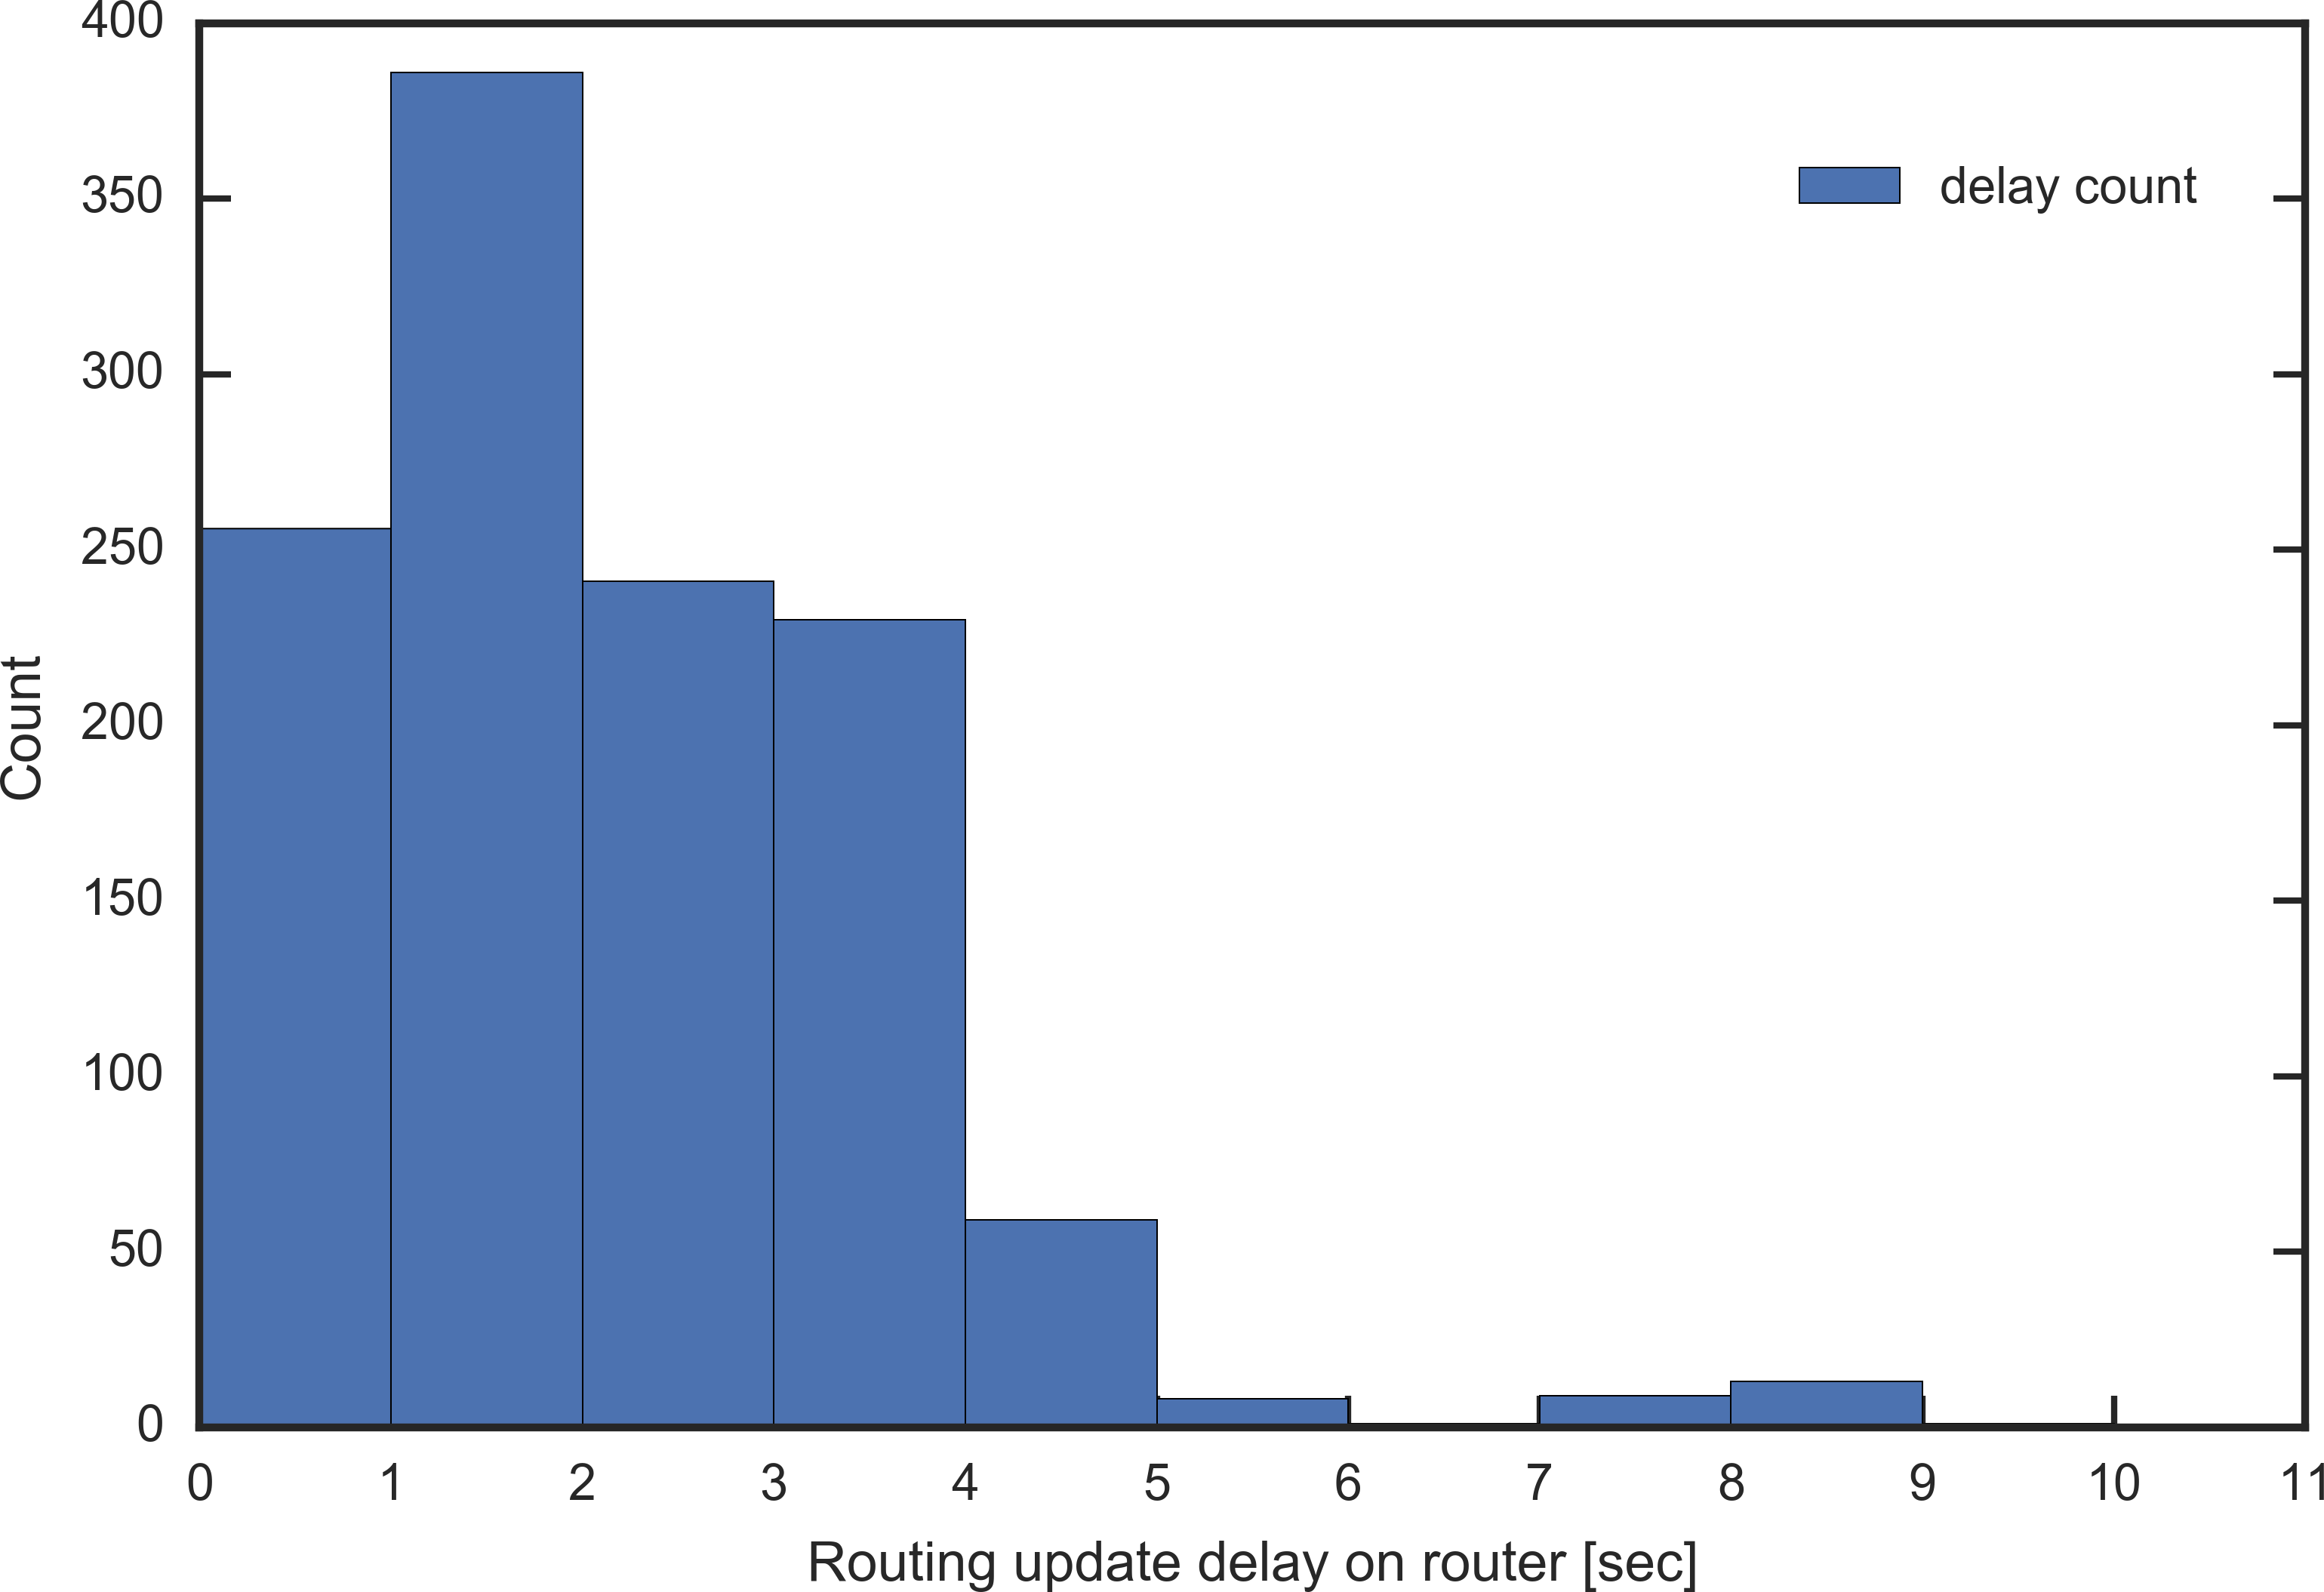
\includegraphics[width=0.9\columnwidth]{Figs/ecmp_delay_histgram}
  \par\bigskip
  \centering
  \begin{minipage}{0.9\columnwidth}
    \caption[ECMP update delay histogram]{
      ECMP update delay histogram.
      This shows the delays until the number of running ipvs pods is reflected in the routing table on the benchmark client, when the number of the ipvs pods is changed randomly every 60 seconds for 20 hours.
    }
    \label{fig:ecmp_delay_histgram}
  \end{minipage}
\end{figure}

The author also carried out throughput measurement to show that the proposed architecture increases the throughput as the number of the load balancers is increased.
Figure~\ref{fig:ecmp_lb_cubic} shows the results of the measurements.
There are four solid lines in the figure, each corresponding to the throughput result when there are one through four of the proposed load balancers.
The saturated levels, i.e. performance levels depend on the number of the ipvs load balancer pods(lb x 1 being the case with one ipvs pods, and lb x2 being two of them and as such). 
The performance level increases linearly as the number of the load balancers increases up to four of the ipvs load balancers, but does not scale further.
This is because the benchmark program uses up CPU power of the benchmark client, i.e., the CPU usage is 100\% when there are more than four load balancers.
The author expects that replacing the benchmark client with more powerful machines, or changing the experimental setup so that multiple benchmark clients can access the load balancers through an ECMP router, will improve the performance level further.

Figure~\ref{fig:ecmp_response} shows the throughput measurement results when the author periodically changed the number of the load balancers. 
The red line in the figure shows the number of ipvs load balancer pods, which is changed randomly every 60 seconds.
The blue line corresponds to the resulting throughput.
As can be seen from the figure, the blue line nicely follows the shape of the red line.
This indicates that new load balancers are immediately utilized after they are created, and after removing some load balancers, the traffic to them is immediately directed to the existing load balancers.

Figure~\ref{fig:ecmp_delay_histgram} shows a histogram of the ECMP update delay, where the author measured the delays until the number of running ipvs pods is reflected in the routing table on the benchmark client, as the number of the ipvs pods is changed randomly every 60 seconds for 20 hours.
As can be seen from the figure, most of the delays are within 6 seconds, and the largest delay during the 20 hours experiment was 10 seconds.
The author concludes that ECMP routing update in the proposed architecture is quick enough.

\FloatBarrier

\section{Summary}\label{Conclusions}

In this chapter, the performance levels of the proposed load balancer have been evaluated. 
The author carried out throughput measurement to verify the feasibility of the load balancer.
The author confirmed that the proposed load balancer is portable, and the ECMP routing is redundant and scalable.

From the throughput measurement of the proposed load balancer using physical servers in the on-premise data center, the author confirmed the followings;
The throughput of the proposed load balancer linearly increases as the number of nginx {\em pod}s increases, and then it eventually saturates, indicating the load balancer functions properly.
The throughput maximum depends on the multicore packet processing settings and overlay network settings.
The throughput increases as the number of CPU cores that are utilized for packet processing increases.
The throughput of the host-gw mode without any encapsulation is higher than vxlan mode and udp mode with encapsulations.
The throughput of the ipvs in a container is equivalent to that of the iptables DNAT as a load balancer, in 1Gbps network environment.
This is due to the bandwidth limitation of the experimental network.
By utilizing ipvs-tun mode, i.e., L3DSR, the throughput of the ipvs container can be further improved, up to 1.5 times.

The author also carried out the same throughput measurement in GCP and AWS to investigate the portability of proposed load balancer.
%to show the containerized ipvs load balancer is runnable even in the cloud environment.
While the performance levels of the proposed load balancers in cloud environments are inferior to those in on-premise data centers, the ipvs container was able to run and functioned properly, in both GCP and AWS.
The author suspects the lesser performance levels in cloud environments are due to the overhead of VMs.

Finally, the author evaluated ECMP functionality by monitoring routing table updates on the router when the new load balancer is added or removed.
The author also measured throughput by changing the number of load balancers.
The ECMP routing update in the proposed architecture is properly functioning and quick enough.
The linear scalability of the ECMP throughput has been confirmed up to 4x of singel load balancer throughput.

The proposed software load balancer is proved to be portable.
The proposed architecture is proved to be redandunt and scalable up to 800K [req/sec].
